\documentclass[11pt,letterpaper,twoside]{report}

% Layout
\usepackage{geometry}
\usepackage{setspace}
\usepackage{titlesec}
\usepackage[subfigure]{tocloft}
\usepackage{multirow}
\usepackage{float}
\usepackage{lscape}
\usepackage{longtable}
% Citation style
\usepackage{natbib}
%\usepackage{apalike}
\usepackage{xpatch}
\setlength{\bibsep}{\baselineskip}
% include citations inline
%\usepackage{bibentry}
%\nobibliography*

% Figures
\usepackage{subfigure}
\usepackage{graphicx}
\usepackage{epsfig}
\usepackage{booktabs}
\usepackage{multicol}
\usepackage{listings}
\usepackage{caption}
%\usepackage{subcaption}

% Math
\usepackage{amsthm}
\usepackage{amsmath}
\usepackage{amssymb}

% Typography
%\usepackage{times}
\usepackage{microtype}
\usepackage{textcomp}

% Macro support
\usepackage{xspace}

% PDF links
\usepackage[hidelinks]{hyperref} % backref=page

\usepackage{titlesec}
\titleformat*{\section}{\fontsize{12}{14}\selectfont}
%\setlength{\bibsep}{20pt plus 0.3ex}

\usepackage{titlesec}

% Use proper margins.
\geometry{letterpaper,left=1in,top=1in,right=1in,bottom=1in,nohead}


% double-space text
\doublespacing

% Center chapter titles, omit page numbers.
\titleformat{\chapter}[display]{\fillast\bfseries}{\Large\MakeUppercase{\chaptertitlename} \thechapter}{-11pt}{\huge\singlespacing}[\thispagestyle{empty}]

% Extend to 2in top margins
% Leave 22pts = 2x font size after heading
\titlespacing{\chapter}{0in}{0.62in}{22pt}

% Indent paragraphs four spaces throughout the thesis/dissertation.
\setlength{\parindent}{4ex}

% Tweak spacing of paragraph labels.
\titlespacing{\paragraph}{0in}{0.08in}{0.07in}

% We want numbered subsubsections
\setcounter{secnumdepth}{3}
\setcounter{tocdepth}{3}

% We need to double-space between footnotes.
\setlength{\footnotesep}{\baselineskip}

% We don't want crazy vertical spacing.
\raggedbottom

% We don't want abandoned words.
\clubpenalty=10000 
\widowpenalty=10000

% Prevent awkward hyphenations.
\hyphenation{Raj-kumar}


% citation style

% default: cite with (Name, year)
\renewcommand{\cite}{\citep}

% common abbreviations
\newcommand{\eg}{{\it e.g.}\xspace}
\newcommand{\ie}{{\it i.e.}\xspace}
\newcommand{\etc}{{\it etc.}\xspace}
\newcommand{\etal}{\emph{et~al}\mbox{.}\xspace}

\newcommand{\xth}{\ensuremath{^{\text{th}}}\xspace}
%\newcommand{\fst}{\ensuremath{^{\text{st}}}\xspace}



\newcommand{\vs}{{vs\mbox{.}}\xspace}

% common Math notation
\newcommand{\NAT}[0]{\mathbb{N}\xspace}
\newcommand{\fun}[1]{\mathit{#1}} % typeset as function name
\newcommand{\setsize}[1]{\left| #1 \right|}
\newcommand{\setdef}[2]{\left\{ #1 \ \left|\  #2\right.\right\}}
\newcommand{\dispsum}[0]{\displaystyle\sum}

\newcommand{\defeq}[0]{\triangleq}
\renewcommand{\mod}{\operatorname{mod}}

% time units
\newcommand{\mus}[0]{\ensuremath{\mu s}\xspace}
\newcommand{\us}[0]{\ensuremath{\mu s}}
\newcommand{\ms}[0]{\ensuremath{\fun{ms}}\xspace}

% algorithm names
\newcommand{\kwfont}[1]{\textsf{#1}\xspace} %\small
% variable name
\newcommand{\var}[1]{\ensuremath{{\fun{#1}}}\xspace} %\small

%http://hstuart.dk/2007/08/03/programming-latex-%E2%80%94-writing-commands/
\newcommand{\mkkw}[2]{
	\newcommand{#1}[0]{\kwfont{#2}}
}

% fancy symbols and functions
\newcommand{\Alg}[0]{{\mathcal A}}
\newcommand{\Test}[0]{{\mathcal T}}
\newcommand{\Mach}[0]{{\mathcal M}}

\newcommand{\usum}[0]{u_{\mathrm{sum}}}
\newcommand{\umax}[0]{u_{\mathrm{max}}}
\newcommand{\umin}[0]{u_{\mathrm{min}}}
\newcommand{\utop}[0]{u_{\mathrm{top}}}

\newcommand{\esum}[0]{e_{\mathrm{sum}}}
\newcommand{\emax}[0]{e_{\mathrm{max}}}
\newcommand{\emin}[0]{e_{\mathrm{min}}}
\newcommand{\etop}[0]{e_{\mathrm{top}}}

\newcommand{\dsum}[0]{\delta_{\mathrm{sum}}}
\newcommand{\dmax}[0]{\delta_{\mathrm{max}}}
\newcommand{\dmin}[0]{\delta_{\mathrm{min}}}
\newcommand{\dtop}[0]{\delta_{\mathrm{top}}}

\newcommand{\prio}[0]{\mathsf Y}
\newcommand{\eprio}[0]{\mathsf y}

% src code
\newcommand{\src}[1]{\textsf{\small #1}\xspace}


% schedulers
\mkkw{\cfs}{CFS}

\mkkw{\edf}{EDF}
\mkkw{\edfwm}{EDF-WM}
\mkkw{\fp}{FP}
\mkkw{\fprm}{RM}
\mkkw{\fpdm}{DM}
\mkkw{\gedf}{G-EDF}
\mkkw{\gsnedf}{GSN-EDF}
\mkkw{\gfp}{G-FP}
\mkkw{\pedf}{P-EDF}
\mkkw{\pfp}{P-FP}
\mkkw{\cedf}{C-EDF}
\mkkw{\pssched}{PS}

\mkkw{\pfsched}{PF}
\mkkw{\pd}{PD}
\mkkw{\pds}{PD$^2$}
\mkkw{\cpds}{C-PD$^2$}

\mkkw{\jlfp}{JLFP}
\mkkw{\jldp}{JLDP}


% Plugins

\mkkw{\pfpgi}{P-FP-Rm}
\mkkw{\pfpdi}{P-FP-R1}
\mkkw{\pedfgi}{P-EDF-Rm}
\mkkw{\pedfdi}{P-EDF-R1}
\mkkw{\cedfiigi}{C2-EDF-Rm}
\mkkw{\cedfiidi}{C2-EDF-R1}
\mkkw{\cedfiiigi}{C6-EDF-Rm}
\mkkw{\cedfiiidi}{C6-EDF-R1}
\mkkw{\gedfgi}{G-EDF-Rm}
\mkkw{\gedfdi}{G-EDF-R1}

\mkkw{\cedfalldi}{C24-EDF-R1}

\mkkw{\capdsiigi}{C2-aPD$^2$-Rm}
\mkkw{\capdsiidi}{C2-aPD$^2$-R1}

\mkkw{\capdsiiigi}{C6-aPD$^2$-Rm}
\mkkw{\capdsiiidi}{C6-aPD$^2$-R1}

\mkkw{\gapdsgi}{G-aPD$^2$-Rm}
\mkkw{\gapdsdi}{G-aPD$^2$-R1}

\mkkw{\cspdsiigi}{C2-sPD$^2$-Rm}
\mkkw{\cspdsiidi}{C2-sPD$^2$-R1}

\mkkw{\cspdsiiigi}{C6-sPD$^2$-Rm}
\mkkw{\cspdsiiidi}{C6-sPD$^2$-R1}

\mkkw{\gspdsgi}{G-sPD$^2$-Rm}
\mkkw{\gspdsdi}{G-sPD$^2$-R1}


% POSIX

\mkkw{\schedfifo}{SCHED\_FIFO}
\mkkw{\schedrr}{SCHED\_RR}
\mkkw{\schedother}{SCHED\_OTHER}
\mkkw{\schedspor}{SCHED\_SPORADIC}
\mkkw{\prioprot}{PRIO\_PROTECT}
\mkkw{\scheddl}{SCHED\_DEADLINE}

% locking protocols
\mkkw{\npcs}{NCP}
\mkkw{\srp}{SRP}
\mkkw{\pcp}{PCP}
\mkkw{\msrp}{MSRP}
\mkkw{\dpcp}{DPCP}
\mkkw{\mpcp}{MPCP}
\mkkw{\mpcpvs}{MPCP-VS}
\mkkw{\fmlp}{FMLP}
\mkkw{\fmlpp}{FMLP$^{\mathrm{+}}$}
\mkkw{\npfmlpp}{NP-FMLP$^{\mathrm{+}}$}
\mkkw{\omlp}{OMLP}
\mkkw{\pip}{PIP}

% RW lock implementations
\mkkw{\pft}{PF-T}   % simple PF RW lock
\mkkw{\pfc}{PF-C}   % compact PF RW lock 
\mkkw{\pfq}{PF-Q}  % queue PF RW lock
\mkkw{\rwlin}{LX-RW}
\mkkw{\tft}{TF-T}
\mkkw{\tfq}{TF-Q}
\mkkw{\mtxt}{MX-T}
\mkkw{\mtxq}{MX-Q}

% locking protocol details
\newcommand{\FQ}[1]{FQ$_{#1}$}
\newcommand{\PQ}[1]{PQ$_{#1}$}

\newcommand{\WQ}[1]{WQ$_{#1}$}
\newcommand{\RQA}[1]{CQ$_{#1}$}
\newcommand{\RQP}[1]{DQ$_{#1}$}
\newcommand{\RQ}[2]{RQ$_{#1}^{#2}$}
\newcommand{\RQi}[1]{\RQ{#1}{1}}
\newcommand{\RQii}[1]{\RQ{#1}{2}}

\newcommand{\KQ}[1]{KQ$_{#1}$}
\newcommand{\KQq}[0]{\KQ{q}\xspace}
\newcommand{\RS}[1]{RS$_{#1}$}
\newcommand{\RSq}[0]{\RS{q}\xspace}

\newcommand{\BQ}[1]{BQ$_{#1}$}

\newcommand{\mc}[0]{\frac{m}{c}}
\newcommand{\nc}[0]{\frac{n}{c}}
\newcommand{\lmax}{L^{\fun{max}}}
\newcommand{\kmin}{k^{\fun{min}}}

% references
\newcommand{\chref}[1]{Chapter~\ref{ch:#1}\xspace}
\newcommand{\chrefs}[2]{Chapters~\ref{ch:#1} and~\ref{ch:#2}\xspace}
\newcommand{\secref}[1]{Section~\ref{sec:#1}\xspace}
\newcommand{\figref}[1]{Figure~\ref{fig:#1}\xspace}
\newcommand{\figrefi}[2]{Figure~\ref{fig:#1}(#2)\xspace}
\newcommand{\tabref}[1]{Table~\ref{tab:#1}\xspace}
\newcommand{\lemref}[1]{Lemma~\ref{lem:#1}\xspace}
\newcommand{\thmref}[1]{Theorem~\ref{thm:#1}\xspace}
\newcommand{\defref}[1]{Definition~\ref{def:#1}\xspace}
\newcommand{\exref}[1]{Example~\ref{ex:#1}\xspace}
\newcommand{\equref}[1]{Equation~(\ref{eq:#1})\xspace}
\newcommand{\inequref}[1]{Inequality~(\ref{eq:#1})\xspace}
\newcommand{\lstref}[1]{Listing~\ref{lst:#1}\xspace}
\newcommand{\pref}[1]{page~\pageref{p:#1}\xspace}
% citations

% resource notation
\newcommand{\res}[0]{\ell}
\newcommand{\req}[0]{\mathcal{R}}
\newcommand{\wreq}[0]{\mathcal{R}^{\fun{W}}}
\newcommand{\rreq}[0]{\mathcal{R}^{\fun{R}}}
\newcommand{\rlen}[0]{{\mathcal L}}
\newcommand{\bspin}[0]{s}

% locking proofs
\newcommand{\tauseq}[0]{\tau^{\fun{seq}}}

% overheads
\newcommand{\evlat}[0]{\Delta^{\fun{ev}}}
\newcommand{\ipilat}[0]{\Delta^{\fun{ipi}}}
\newcommand{\reloh}[0]{\Delta^{\fun{rel}}}
\newcommand{\schedoh}[0]{\Delta^{\fun{sch}}}
\newcommand{\cxsoh}[0]{\Delta^{\fun{cxs}}}
\newcommand{\cpmdoh}[0]{\Delta^{\fun{cpd}}}
\newcommand{\cidoh}[0]{\Delta^{\fun{cid}}}
\newcommand{\tickoh}[0]{\Delta^{\fun{tck}}}

\newcommand{\inoh}[0]{\Delta^{\fun{in}}}
\newcommand{\outoh}[0]{\Delta^{\fun{out}}}

\newcommand{\sysinoh}[0]{\Delta^{\fun{sci}}}
\newcommand{\sysoutoh}[0]{\Delta^{\fun{sco}}}


\newcommand{\numres}[0]{{n_r}}

% complicated names
\newcommand{\litmus}{LITMUS$^{\mathrm{RT}}$\xspace}
\newcommand{\aquo}{AQuoSA\xspace}
\newcommand{\prt}{PREEMPT\_RT\xspace}
\newcommand{\livlin}{L$^4$Linux\xspace}

% parameters

\newcommand{\pacc}[0]{\var{pacc}}
\newcommand{\wratio}[0]{\var{wratio}}

% special footnotes

% from http://help-csli.stanford.edu/tex/latex-footnotes.shtml
\long\def\symbolfootnote[#1]#2{\begingroup%
\def\thefootnote{\fnsymbol{footnote}}\footnote[#1]{#2}\endgroup}

% Theorems, etc.

\newtheoremstyle{mylemthm}% hnamei 
        {6pt}% hSpace abovei 
        {3pt}% hSpace belowi 
        {\slshape}% hBody fonti 
        {}% hIndent amounti1
        {\bfseries}% hTheorem head fonti 
        {.}% hPunctuation after theorem headi 
        {.5em}% hSpace after theorem headi2
        {}% hTheorem head spec (can be left empty, meaning `normal')i

\theoremstyle{mylemthm}

\newtheorem{theorem}{Theorem}[chapter]
\newtheorem{lemma}{Lemma}[chapter]

%\theoremstyle{definition}

\newtheoremstyle{mydef}% hnamei 
        {3pt}% hSpace abovei 
        {3pt}% hSpace belowi 
        {\normalfont}% hBody fonti 
        {}% hIndent amounti1
        {\bfseries}% hTheorem head fonti 
        {.}% hPunctuation after theorem headi 
        {.5em}% hSpace after theorem headi2
        {\thmname{#1} \thmnumber{#2}\thmnote{#3}}% hTheorem head spec (can be left empty, meaning `normal')i

\theoremstyle{mydef}


%% Flush words right at end of paragraph.
%% From: http://tex.stackexchange.com/questions/16330/hfill-after-linebreak
\newcommand\rightparend[1]{{%
      \unskip\nobreak\hfil\penalty50
      \hskip2em\hbox{}\nobreak\hfil\textbf{#1}%
      \parfillskip=0pt \finalhyphendemerits=0 \par}}


\newtheorem{definition}{Definition}[chapter]
\newtheorem{xxexample}{Example}[chapter]

%% "inherent" from xxexample, but place box at the end of example.
\newenvironment{example}{
\begin{xxexample}
}{
\rightparend{$\Diamond$}
\end{xxexample}
}
% \qed   \sqbullet \blackdiamond \vartriangleleft

 %no changes needed here--this is formatting

\begin{document}

% Title page, TOC, etc.

% front matter pages use 2in top margin
\newgeometry{left=1.25in,top=2in,right=1.25in,bottom=1in,nohead}
\pagenumbering{roman}

%1. Title Page

\begin{titlepage}
\begin{center}

% 1. The title of the thesis/dissertation, centered 2� below the top of the page

\vspace{2in}
\begin{singlespace}

THE MODERATING EFFECTS OF THE NEED FOR MULTINATIONAL INVESTMENT ON STATE REPRESSION
 \end{singlespace}


% 2. Your name, centered 1� below the title.
\vspace{61pt} % 1 in = 72pt, 11pt for the line with text
\large Steven W. Saroka
\end{center}


%3. The following statement, within the full mar- gins, 1� below your name:
%�A dissertation [or thesis] submitted to the faculty of the University of North Carolina at Chapel Hill in partial fulfillment of the requirements for the degree of	in the Department [or School or Curriculum] of      .�

\vspace{50pt}
\begin{singlespace}
\noindent \large
A thesis submitted to the faculty of the University of North Carolina at Chapel Hill
in partial fulfillment of the requirements for the degree of Master of Arts in
the Department of Political Science.
\end{singlespace}


%4. On the lower half of the page, centered, the words �Chapel Hill�
%and one line below that, the year in which your committee approves
%the completed thesis/dissertation.
\vspace{50pt}
\begin{center}
\begin{singlespace} \large
Chapel Hill\\
2020
\end{singlespace}
\end{center}

%5. On the right-hand side of the page, �Approved by,� followed by lines for the
%signatures of the adviser and four (two for thesis) readers. List

\vspace{50pt}
\begin{flushright}
\begin{minipage}{1.4in} \large
Approved by:\\
Navin A. Bapat \\
Stephen E. Gent \\
Mark J. Crescenzi \\
\end{minipage}
\end{flushright}

\end{titlepage} %did this

%2. Copyright Page (optional)
\newgeometry{left=1.25in,top=8.33in,right=1.25in,bottom=1in,nohead}

%If you wish to copyright your thesis, you must include a copyright page with the following information single-spaced and centered on the bottom half of the page:
%� Year 
%Full Name (exactly as it appears on the title page) 
%ALL RIGHTS RESERVED
%This page should immediately follow the title page, and should bear the lower case Roman numeral: ii.

\begin{center}
\begin{singlespace}
\copyright 2020\\
Steven W. Saroka\\
ALL RIGHTS RESERVED
\end{singlespace}
\vspace*{52pt}
\end{center}

\clearpage
 %did this
\newgeometry{left=1.25in,top=2in,right=1.25in,bottom=1in,nohead}

%3. Abstract

% Normal pages from here on out; TOC title takes care of 2in requirement.
\restoregeometry

%The word �Abstract� should be centered 2? below the top of the page. 
%Skip one line, then center your name followed by the title of the 
%thesis/dissertation. Use as many lines as necessary. Centered below the 
%title include the phrase, in parentheses, �(Under the direction of  
%_________)� and include the name(s) of the dissertation advisor(s).
%Skip one line and begin the content of the abstract. It should be 
%double-spaced and conform to margin guidelines. An abstract should not 
%exceed 150 words for a thesis and 350 words for a dissertation. The 
%latter is a requirement of both the Graduate School and UMI's 
%Dissertation Abstracts International.
%Because your dissertation abstract will be published, please prepare and 
%proofread it carefully. Print all symbols and foreign words clearly and 
%accurately to avoid errors or delays. Make sure that the title given at 
%the top of the abstract has the same wording as the title shown on your 
%title page. Avoid mathematical formulas, diagrams, and other 
%illustrative materials, and only offer the briefest possible description 
%of your thesis/dissertation and a concise summary of its conclusions. Do 
%not include lengthy explanations and opinions.
%The abstract should bear the lower case Roman number ii (if you did not 
%include a copyright page) or iii (if you include a copyright page).

\begin{center}
\vspace*{52pt}
{ABSTRACT}
\vspace{11pt}

\begin{singlespace}
Steven W. Saroka: The Moderating Effects of the Need for Multinational Investment on State Repression \\
(Under the direction of Navin A. Bapat)
\end{singlespace}
\end{center}

What are the effects of resource endowments on state repression? This paper theorizes that states are more likely to engage in repression to secure resource-rich areas to maximize the state’s profits, with repression intensity varying by whether the resource requires outside investment to extract. Should resource extraction require outside investment, states must restrain their repression and share profits with an external multinational corporation. This theory yields predictions that there will be higher levels of state repression closer to sites of natural resources, and that overall levels of repression will be lower in areas with resources that require multinational investment than in areas with resources that the state can extract with its own capabilities. This is tested using a logit model and PRIO-GRID cell-years and repression data from the UCDP's Georeferenced Event Dataset.


\clearpage
 %did this

%4. Dedication, Acknowledgement(s) and/or Preface (all optional)

%%A dedication is an honorific statement from the author to a person or group to 
%whom the author commends the effort and product of the dissertation. Most 
%dedications are short statements of tribute beginning with �To��. No heading is 
%required on the dedication page. The text of short dedications should be 
%centered between the left and right margins and 2? from the top of the page.

\begin{center}
\vspace*{52pt}
Dedication\ldots
\end{center}

\pagebreak

%Acknowledgements are the author's statement of gratitude to and
%recognition of the people and institutions who helped the author's
%research and writing.

\begin{center}
\vspace*{52pt}
{ACKNOWLEDGEMENTS}
\end{center}

I want to thank the many people who provided input, suggestions, and help on this thesis. I am indebted to Navin Bapat for his guidance and insight throughout this project, as well as to Stephen Gent and Mark Crescenzi for their very helpful criticisms and comments. Additionally, I would like to thank Simon Hoellerbauer and Ted Enamorado for their endless patience and help with coding in R. 

\clearpage
 %did this

%\begin{center}
{\Large \textbf{PREFACE}}
\end{center}

Suspendisse semper, nibh at dignissim volutpat, nibh lacus tempus augue, nec tempus est leo nec sem. Phasellus eros felis, malesuada nec, lobortis quis, posuere in, risus. Cras sagittis accumsan purus. Nullam nulla nisl, ultrices a, lacinia eu, lacinia vitae, risus. Donec varius lorem. Nam nisl. Vivamus non augue. Vestibulum dignissim auctor neque. Ut vel eros. Aenean tempor, erat vel feugiat porta, nunc justo euismod dui, ut hendrerit dolor lusto sit amet tortor. Nunc adipiscing massa in erat. Proin tincidunt tellus vitae augue consequat suscipit. Aliquam feugiat libero non odio. Fusce adipiscing augue ac arcu. In orci. Cras lobortis euismod libero.
\tbw


\clearpage





%5. Table of Contents, with page references
\renewcommand{\contentsname}{TABLE OF CONTENTS \hfill}  
%\renewcommand{\contentsname}{TABLE OF CONTENTS}
\renewcommand{\cfttoctitlefont}{\hfill}
\renewcommand{\cftaftertoctitle}{\hfill}
\renewcommand{\cftdotsep}{1.5}
\cftsetrmarg{1.0in}

\setlength{\cftbeforetoctitleskip}{61pt}
\setlength{\cftaftertoctitleskip}{28pt}

% format chapter entries like other entries
\renewcommand{\cftchapfont}{\normalfont}
\renewcommand{\cftchappagefont}{\normalfont}
\renewcommand{\cftchapleader}{\cftdotfill{\cftdotsep}}

\setlength{\cftbeforechapskip}{15pt}
\setlength{\cftbeforesecskip}{10pt}
\setlength{\cftbeforesubsecskip}{10pt}
\setlength{\cftbeforesubsubsecskip}{10pt}

\begin{singlespace}
\tableofcontents
\end{singlespace}


\clearpage
 %no changes needed here, apparently, since this is generated automatically


%6. List of Tables, with titles and page references (if applicable)

\renewcommand{\listtablename}{LIST OF TABLES}
\phantomsection
\addcontentsline{toc}{chapter}{LIST OF TABLES}

\setlength{\cftbeforelottitleskip}{-11pt}
\setlength{\cftafterlottitleskip}{22pt}
\renewcommand{\cftlottitlefont}{\hfill}
\renewcommand{\cftafterlottitle}{\hfill}

\setlength{\cftbeforetabskip}{10pt}

\begin{singlespace}
\listoftables
\end{singlespace}

\clearpage
 %no changes needed here for same reason


%7. List of Figures or Illustrations, with titles and page references (if applicable)

\renewcommand{\listfigurename}{LIST OF FIGURES}
\phantomsection
\addcontentsline{toc}{chapter}{LIST OF FIGURES}

\setlength{\cftbeforeloftitleskip}{-11pt}
\setlength{\cftafterloftitleskip}{22pt}
\renewcommand{\cftloftitlefont}{\hfill}
\renewcommand{\cftafterloftitle}{\hfill}

\setlength{\cftbeforefigskip}{10pt}
\cftsetrmarg{1.0in}

\begin{singlespace}
\listoffigures
\end{singlespace}
\clearpage
 %no changes needed here for same reason

%8. List of Abbreviations (if applicable)
%\phantomsection
\addcontentsline{toc}{chapter}{LIST OF ABBREVIATIONS}

\begin{center}
{\Large \textbf{LIST OF ABBREVIATIONS}}
\end{center}

\newcommand{\Ab}[2]{\noindent  #1 \> #2 \\}
\newcommand{\Abi}[2]{\noindent #1 \hspace{1.5cm} \= #2 \\}

\begin{tabbing}
\Abi{ABD}{All But Dissertation}
\Ab{I/O}{Input/Output}
\Ab{IPC}{Inter-Process Communication}
\Ab{IPI}{Inter-Processor Interrupt}
\Ab{WSS}{Working Set Size}
\Ab{AYO}{Add Your Own in alphabetic order\ldots}
\end{tabbing}

\clearpage


%9. List of Symbols (if applicable)

\pagenumbering{arabic}
 %all updated

\vspace*{25pt}
\section*{\hfill INTRODUCTION \hfill}
%\chapter*{Introduction}
\addcontentsline{toc}{chapter}{INTRODUCTION}

When and how do resource endowments contribute to state repression? Anecdotal evidence suggests undertheorized variation, as illustrated by the contrasting cases of Nigeria and Zimbabwe. In Nigeria’s southern Niger Delta region, the site of the state’s oil reserves, grievances regarding the state’s failure to share the benefits of oil wealth enabled the rise of a mixture of criminal and insurgent groups. In particular, the rise of the Movement for the Emancipation of the Niger Delta (MEND) in 2006 was marked by an insurgent focus on attacking oil-related facilities and kidnapping associated personnel \cite{Asuni19,ICG06}. A counterinsurgency campaign was followed in 2009 by a government amnesty, which led to an increase in oil production, but failed to prevent the rise of another insurgent group, the Niger Delta Avengers, in 2016 \cite{BBC,Forbes}. While the details of this insurgency are more complex \cite{Nwankpa14,AghedoOsumah15}, this case is notable for the government attempts to repress and, when repression was unsuccessful, negotiate with insurgents who were threatening the extraction of potentially lucrative resources. Despite the ultimately temporary nature of the bargain, this outcome still sharply contrasts with government action in Zimbabwe. There, the discovery of the Marange diamond deposits in 2006 was followed by efforts by the national government to exclude foreign companies from investment in these deposits, in favor of state-owned companies. A diamond rush was followed by police repression beginning in late 2006, with military units moving into the area in 2008 and overseeing continued repression and forced civilian labor \cite{HRW09}. 


The contrast of an amnesty in Nigeria with continued repression in Zimbabwe raises a question: what caused the variation in strategies employed by the state in these two cases? Why did the government of Nigeria ultimately offer an amnesty while the government of Zimbabwe continued its repression? More generally, when and how do resources influence a controlling state’s decision to repress its citizens or restrain itself? In this paper, I develop a theory of state repression as a means of consolidating control over resource-rich areas with the ultimate aim of profiting from those resources. As different kinds of resources require different levels of outside investment from multinational corporations to extract and thus profit from them, states may restrain their use of repression with the goal of attracting the necessary outside investment to enable resource extraction and maximize the profits from these resources. This theory yields two hypotheses that I test empirically using data on state repression and resource locations. This theory receives support, and I close with a discussion of potential improvements and extensions for future work.

       
\newpage
\vspace*{25pt}
	\section*{\normalfont \hfill LITERATURE REVIEW \hfill}
	\addcontentsline{toc}{chapter}{LITERATURE REVIEW}

The study of natural resources and state repression has, over time, become closely linked to a literature on both internal conflict and the effects of resources on rebellion. While extant work has naturally focused on geographic factors such as resource location and structural factors such as economic incentives for engaging in conflict, this review of the literature also highlights undertheorized elements of this story, particularly with regards to the differing profitability of different resources, as well as a lack of substantial consideration of the role of multinational investors. I review each of these aspects of the literature in turn, before closing with a summary of the gaps revealed by this literature that my theory is intended to fill.

The linkage of natural resources and suboptimal governance outcomes, such as state repression or civil war, is not necessarily new. Relatively early work such as Le Billon (\citeyear{LeBillon01}) argued that resources could become integrated into the political economy of conflicts, as opposing actors attempt to exploit them, but that specific social processes drive a society’s risk of war due to resources. Ross (\citeyear{Ross01}), by contrast, generalized by arguing that the resource curse in oil-producing states was due to rentier state effects; this theoretical development drew on earlier work on state development as arising from bargaining between tax-seeking governments and citizens whom they wished to tax \cite{BatesLien85}. A review of research in this area by Ross (\citeyear{Ross15}) finds that a resource curse effect exists for petroleum, as its income makes authoritarian regimes more durable while increasing the probability of some kinds of corruption. Additionally, both petroleum and other resources may trigger or prolong conflict in low- or middle-income states. However, Ross (\citeyear{Ross15}) notes that there is a general lack of consensus regarding the precise causal mechanisms behind the resource curse, and why this literature has relatively strong findings for petroleum but weak or contradictory findings for other kinds of natural resources. Why these findings differ across resource types remains unexplored, and this is a gap I seek to remedy with my theory.

There is also a substantial literature on state repression; while earlier work often focused on assorted state-level predictors of repression, more recent work here has linked natural resources and state repression. A general definition of state repression is given by deMeritt: “the threat to subdue or act of subduing someone by institutional or physical force. Political violence is a particular form of repression involving the threat to use or actual use of physical force to achieve political goals” \cite[p.~2]{deMeritt16}. Notably, she states that “repression and political violence are strategic policies that governments employ in pursuit of important political and/or military objectives. The most fundamental of these objectives is the maintenance of control” \cite[p.~2]{deMeritt16}. This definition of repression matches well with that of Besley and Persson (\citeyear{BP09}), who define state repression as one-sided violence by the state. Early cross-national studies focused on democracy levels, social inequality, and economic growth as meaningful predictors of state repression \cite{Henderson91,Davenport95}. Later work added nuance to this, noting that the beneficial effects of democracy may have relatively small effect sizes compared to conflict, either civil or interstate \cite{Davenport04}. Additionally, autocratic regimes are not necessarily monolithic in their repression efforts, with single-party autocracies repressing less than other autocracies \cite{Davenport07}. Davenport’s work is also notable for proposing the “Law of Coercive Responsiveness,” which argues that state repression is a response by governments to perceived threats \cite{Davenport07b}. Besley and Persson (\citeyear{BP09}) identified poverty, rents from natural resources, and weak political institutions as root causes of political violence; the overlap between these factors and the resource curse literature indicates a linkage of these two phenomena.

Some scholars have argued that extant work has failed to fully model the strategic nature of state repression and dissent in the form of popular protests \cite{Pierskalla10}. Specifically, Pierskalla argues that this failure is why tests of the effectiveness of government repression in suppressing popular protest have found a range of relationships with no clear consensus. Similarly, Ritter and Conrad (\citeyear{rc2016}) argue that preexisting work on anti-government dissent and government repression has failed to adequately grapple with their endogeneity, as strategic dissidents and governments consider each other’s expected responses before acting. To address this, they use rainfall as an instrumental variable, finding that where states engage in preventative repression, there are no significant effects of dissent on responsive repression. Additionally, violence may not always be a successful tool of repression, and has potential to backfire on governments using it \cite{Suttonetal14}. Ritter (\citeyear{Ritter14}) elaborates on this by using a formal model to show that the reciprocal nature of dissent and repression indicates that the same independent variable can have divergent effects. She finds that while increased job security for executives decreases the probability of repression occurring, it increases the severity of any repression that does occur. Finally, Chenoweth, Perkoski, and Kang (\citeyear{Chenowethetal17}) find in a review of both the state repression literature and the more practice-focused nonviolent resistance literature that regime type conditions scope and intensity of repression, with states over a democratic threshold much less likely to repress.

Approaching the linkage of resources and contentious politics from a different angle, other scholars have drawn linkages between resource wealth and its ability to fuel conflict by both motivating rebellion and potentially funding it. Early work by Collier and Hoeffler (\citeyear{CoHo98, CoHo04}) emphasized the role of economic factors in influencing the viability of engaging in civil war, theorizing that the lure of economic gains from conflict or the low opportunity costs of engaging in it may provide sufficient impetus for civil war. These findings were supplemented by country-level analysis, such as Fearon and Laitin’s (\citeyear{FL3}) focus on favorable conditions for insurgency as predictors of civil war. They emphasized the permissive role of a weak central government as well as enabling factors such as rough terrain and rebel knowledge of a local population sufficiently large to conceal them. Echoing work on the resource curse, however, the precise causal mechanisms underlying these findings were initially unclear \cite{Humphreys05}. Weinstein (\citeyear{Weinstein07}) helped to fill this gap, arguing that resource availability impacted the types of recruits who joined nascent rebel groups, with resource-rich groups attracting more opportunistic recruits while resource-poor groups were forced to rely on social endowments. These recruit types then influenced organizational discipline, ultimately impacting treatment of civilian populations under their control. In a related fashion, others such as Reno (\citeyear{Reno02}) argued that economically successful actors may respond to the collapse of the formal state and its patronage networks by becoming well-armed insurgents, with the prospect of personal economic gain enabling them to recruit individuals who would otherwise have joined more reformist movements. Similarly, Bates argued that the breakdown of political order (including the occurrence of civil war) seen in the African context by the close of the twentieth century was due to the failure of a prior equilibrium bargain between citizens and violence specialists which, if upheld, supported stable political order \cite{BGS02, Bates08}. The breakdown of this bargain, according to this framework, led many elites to perceive violent predation as more profitable than upholding existing political institutions and bargains. 

Other scholars have used exogenous price shocks to estimate the impact of resources on conflict. Angrist and Kugler (\citeyear{AK08}) use an exogenous upward shift in coca cultivation and its price in Colombia as a natural experiment to test the link between illegal resource cultivation and civil conflict. They conclude that increased coca growth led to limited economic gains for some actors in some regions, but also to worsened conditions of violence in those same regions. Other scholars have also reported similar findings in the Colombian context \cite{DV13,CD17}. While this focus on a specific type of resource would appear to threaten generalizability, other findings have been congruent with this. With regards to oil, scholars find that the discovery of oil fields can increase the probability of conflict \cite{LM14}. Finally, Berman, Couttenier, Rohner and Thoenig (\citeyear{BCRT17}) find that increased market prices for minerals both increase conflict risk and allow rebel groups to engage in both more and wider-ranging violence by providing a source of financing. 

Finally, there has also been substantial work on the intersection of repression and civil conflict. This literature has emphasized the relationship between them, showing that state repression can be both used by the state in an attempt to preemptively suppress potential dissenters, as well as a tool of conflict should the state face armed rebellion. Cunningham, Gleditsch, and Salehyan (\citeyear{Cunninghametal09}) examine civil war duration and outcome by disaggregating both rebel capacity and state repression, arguing rebel strength can be disaggregated into offensive and defensive military capabilities, while a state’s repression ability can also vary by location within a state, with lessened ability at the periphery. They argue that strong rebels cause conventional-looking conflicts with decisive military outcomes, while weak rebels can prolong a civil war by hiding at the periphery of the state. Elaborating on this theme, Danneman and Ritter (\citeyear{DannemanRitter14}) find that in response to civil war occurring in neighboring states, state authorities will engage in preemptive repression to prevent the diffusion of civil war into their own state, as they anticipate civil war externalities will change the incentives of potential rebels. They argue that state authorities ultimately repress in an attempt to avoid the fate of their warring neighbors. Should they fail to prevent rebellion, Fjelde and Hultman (\citeyear{FH14}) find that conflict actors such as states may use ethnicity as a collective targeting cue, engaging in violence against civilians in an attempt to deprive the rebel movement of its civilian support. As such, states may engage in civilian targeting as a strategic form of repression. Empirical evidence shows that governments may turn to mass killings as a strategy to remove bases of insurgent support \cite{VHB04}, while Zhukov’s (\citeyear{Z17}) historical work finds that the amount of violence against civilians in German-occupied Belarus was dependent on the extent to which combatants depended on local or external sources of support.

This review of the literature shows that while resources and violence in the form of state repression and civil war are linked, with resources increasing both the incentives of rebels to go to war and their strength once conflict has begun and the incentives of governments to engage in violence to secure these resources, the strategic use of state repression as it relates to the control of valuable resources remains an undertheorized area. Throughout this literature, studies of repression often implicitly treat repression as distributed evenly throughout a state—when the effects of state repression are considered, the specific locations of that repression are often not taken into account, meaning that analyses do not explain why states simultaneously engage in repression in one region but not in another. This leaves undertheorized the question of whether the presence of resources influences a state’s decision to use repression in a given area. A second, related question concerns why states vary in their repression. To return to my opening examples, why was there continued repression in Zimbabwe while Nigeria eventually turned to negotiation? In the next section, I answer these questions with a theory of resource type variation and government repression incentives.

\newpage
\vspace*{25pt}
\section*{\normalfont \hfill THEORY \hfill}
\addcontentsline{toc}{chapter}{THEORY}

Given this literature, it seems a reasonable starting assumption that states use internal repression as a means of consolidating control over territory and any resources it may contain. For the sake of parsimony, this theory treats the state as a unitary actor. An implicit assumption regarding repression that applies throughout the rest of this paper, and also forms an important scope condition of this theory, is that the state's monopoly on the use of force means that the state is always using or threatening some level of force against its population \cite{tilly1975}. I make no initial assumptions about the amount or type of repressive force used: a state may use the bare minimum necessary to enforce its laws via police action, or engage in more draconian repressive action such as mass killings.

Another important opening consideration is that not all territory contains natural resources of equal value. Resources are usually not uniformly distributed over a state’s territory, as geological processes lead to concentrations of minerals or oil in some areas but not others. This haphazard distribution is compounded by the need to discover natural resources. Previously undiscovered natural resources can be found by accident or prospecting efforts, introducing a further element of chance to a state’s known distribution of natural resources as certain resource concentrations may be overlooked. Additionally, market values for resources are prone to fluctuation, as demonstrated by global oil markets, leading to variations in value of resources across resource types and over time. 

As a state can use internal repression as a means of consolidating control over areas with known resources within its borders, this implies that the state must have some motive for consolidating its control. In this theory, I adopt the assumption that states wish to maximize the profits they accrue from natural resources within their territory. Control of those natural resources is a necessary prerequisite for that goal, though not necessarily a sufficient condition for it—a point to which I return below in the discussion of resource types. Here, these starting considerations imply that a state’s incentives to engage in repression against its citizens will vary by location. While states may engage in different amounts of repression in different areas for a variety of reasons, such as preexisting unrest in one region but not in another, I theorize that holding those other motivations constant, the presence of exploitable resources of any kind should predict relatively higher levels of state repression in order to secure the area, and thus those resources, for the direct benefit of the state. Theoretically, this repressive violence is solely motivated by the state’s desire to secure the maximum amount of resource profits for itself, and so should not be conditional on the type of resource under consideration, as all resources have at least some value. Additionally, this indicates an implicit sharp decline in the explanatory power of this mechanism as the distance between an incident of repression and the closest site of natural resources increases, as the motivation for repression due to the presence of a resource should fade as the proximity to that resource diminishes. This suggests a first, general hypothesis:

\begin{itemize}
	\item \textbf{H1:} There will be more state repression closer to sites of natural resources.
\end{itemize}

However, this theory is further complicated by variation in the level of outside investment from multinational corporations required for the state to enjoy the profits from a given resource. Some resources may require little or no outside investment before the state can extract and profit from them, while others may require substantial external investment. In these latter cases, this requirement for external investment may place these resource profits beyond the reach of the state by itself \cite{rossbook,colganbook}. However, this access can be facilitated by multinational corporations committing substantial capital and personnel to extractive ventures. If so, this implies that a reasonable state lacking such extractive capacity must consider the investment incentives of such external investors when choosing its actions, including its level of repression—in short, the state must consider how best to attract investment. This involves a brief consideration of the preferences of these external investors, a term which I use synonymously with multinational corporations. For the sake of theoretical simplicity, this theory assumes that these corporations are profit-seeking, but also wish to avoid substantial risk to their personnel or corporate assets \cite{BSY14}, such as physical damages due to popular unrest or outright expropriation of production facilities by the state’s government. These investors have no fundamental preferences over state repression or lack thereof—their primary concerns are with the profitability of the venture and the security of their assets.

Thus, this kind of external investment is only necessary in cases where resource extraction would require the provision of large amounts of external investment and expertise, which the state may be unable or unwilling to provide\footnote{This condition covers states at all levels of development: while developing states may lack the funding or human capital, developed states may not wish to provide such funding if the private sector can assume the costs and risks of such an operation.}. For the purposes of illustration for the rest of this section, and to match with the later operationalization in my empirical analysis, I conceptualize of this difference in required investment through reference to two archetypal resources, which are often discussed in terms of being lootable and not lootable (terms I treat as synonymous with easy- and hard-to-extract): diamonds and oil. Diamonds are here theorized to require little to no outside investment before they can be extracted and sold, as they can be mined with relative ease compared to extracting oil deposits. Oil deposits, by contrast, require substantial investment into the drilling and extraction infrastructure necessary to both extract the oil and transport it to market. Thus, profits from diamonds (or other easy-to-extract resources) can be obtained by the state with minimal regard for outside investors, as they are not necessary for the state to enjoy the profits from these resources. By contrast, profits from oil reserves (or other hard-to-extract resources) cannot be obtained by most states, especially those that are still developing, without substantial outside investment. 

This variation in the need for outside investment also ultimately solves what at first seems to be a potentially intractable commitment problem implied by the incentives of this theory: the clash between the desire of the state to maximize the profits from its resources and the desire of the firm to maximize its own profits from its investment, given that the state may use repressive violence to seize control of resources and thus deprive the firm of value. However, so long as the state requires the expertise of the firm to extract these resources, and thus to derive any substantial profits from them, the state has differential incentives to repress in resource-rich areas based on the type of resources: those areas with resources that require outside investment will experience minimal amounts of repression, as the state must avoid scaring away firms that may fear violent repression will be used to expropriate their assets, while those areas with resources that do not require such investment will experience higher amounts of repression as the state can directly seize resources for itself without fearing a loss of profits.

To summarize, this theory argues that profit-maximizing states, seeking to maximize the profits from the resources within their territory, face different incentive structures for their choices conditional on the type of resources they wish to exploit. When considering lootable and easy-to-extract resources, states have no need to consider whether their behavior will deter potential investors, as the presence of those investors is not necessary for the state to maximize its profits. As such, they will be free to engage in repressive violence in these cases to secure these resources. Such violence will be especially incentivized if the state fears a rebel group is also seeking to control these resources, and wishes to seize them before a rebel group does. By contrast, if the state is considering non-lootable resources that are difficult to extract, and thus require the investment of outside firms to enable their extraction and maximize their profitability, states are aware that investors will be unwilling to invest in an area where repression or outright civil war would endanger their assets or extractive efforts. States are aware that they cannot simply seize all profits from these resources for themselves, but must share them with these outside investors if they wish to gain their cooperation and thus a share of the profits—that is, they must avoid engaging in repression against investors and their personnel intended to seize sole control of the resource, which would drive off the investor and leave the state with no profits. Additionally, if they are facing rebel violence, they may attempt to pacify the rebellion via negotiation in order to minimize violence. In this case, the state maximizes its profits by restraining its predation. 

This logic suggests, fundamentally, that states will seek to establish ownership via repression in areas containing resources that do not require outside investment to extract, but will engage in lower levels of repression in areas with resources that do require outside investment. In this way, the necessary presence of multinational corporations can incentivize more peaceful outcomes, as their necessity restrains the state’s level of repressive violence—ultimately, resource type drives state repression or the lack thereof. This indicates that repression should roughly be a function of whether states require international investment to profit from their resources: repression will be lower if they do, and higher if they do not. To restate this in terms of the oil and diamond resources, this implies that states will engage in less repression in areas containing oil than in those containing diamonds. This indicates a second hypothesis:

\begin{itemize}
	\item \textbf{H2:} Overall levels of repression will be lower in areas containing hard-to-extract resources than in areas containing easy-to-extract resources.
\end{itemize}

\newpage
\vspace*{25pt}
\section*{\normalfont \hfill METHODS \hfill}
\addcontentsline{toc}{chapter}{METHODS}
Testing these hypotheses quantitatively requires both data that reflects the key elements of this theory and statistical models that can accurately estimate the types of data being used. This implies several requirements for any research design. First, and most fundamentally, there is a requirement for data on resource locations and incidents of state repression, as both of these are crucial variables in the theory. Second, due to the importance of geographic proximity in this theorized relationship between state repression and resource locations, these data sources must have some embedded means of providing information on the geographic closeness of these two phenomena. Without some way of linking the two, any analysis would risk finding spurious relationships between resources and incidents of repression that were located in different parts of the world. Third, to avoid selection on the dependent variable, there must be variation in the occurrence of state repression within whatever unit of analysis is used. Fourth, these data sources must be able to be examined quantitatively. Fifth, these data must have broad geographic and temporal coverage, as the theory does not bound itself to specific regions or periods of history. To fulfill these requirements, I combine the civilian casualty information from incidents of state repression in the UCDP's Georeferenced Event Dataset \cite{SundbertMelander13} with the Peace Research Institute Oslo's (PRIO's) PRIO-GRID dataset \cite{priogridcode}. This enables me to test my hypotheses using a logit model. In the following sections, I first describe the data sources from which I created my dataset, before presenting some descriptive statistics from the dataset. I then present and elaborate upon the results of the logit model.

The UCDP's Georeferenced Event Dataset \cite{SundbertMelander13} covers 1989-2018, with global (excepting Syria) coverage during that time \cite{Stina19}. PRIO-GRID contains information on the presence of both oil and diamond deposits within the approximately 55 by 55 kilometer grid cells that comprise that dataset, with global coverage for the world’s landmasses \cite{LRT7,Gilmore5,LGG5}. From the Georeferenced Event Dataset, there is information on the number of deaths from incidents of one-sided violence\footnote{Notably, some incidents contained 0 deaths according to the UCDP’s best estimate.} committed by governments against their civilian population per year within each PRIO-GRID cell, as well as a binary indicator of whether those occurred during an active conflict-year as defined by the UCDP\footnote{This binary indicator takes a value of 1 if the grid cell-year experienced any active conflicts as defined by the UCDP, which are state-based conflict, non-state conflict, and one-sided violence \cite{Stina19}. This ensures that this indicator accurately reflects whether there is any substantial violence occurring in the cell-year, not just whether one-sided violence was perpetrated by the government during that cell-year, which would prevent the use of this as a control for civil wars.}. By construction of the GED, the victims of one-sided government violence are always civilians; this dataset does not, for example, include combatant deaths from conflict with insurgent groups, and so there is no concern that other types of violence are being erroneously included in this analysis. I operationalize state repression as incidents of one-sided violence in this dataset where the perpetrator was the government. As this dataset was built to be compatible with the PRIO-GRID dataset, this enables me to generate a cell-year tally of civilian deaths within each cell for each year, that I then match with the PRIO-GRID cells. Notably, while the Georeferenced Event Dataset has coverage from 1989-2018, the PRIO-GRID dataset only contains coverage from 1946-2014, with selected variables within it covering fewer years within that range. My unit of analysis is thus the grid cell-year.

I include a binary indicator variable for whether a cell-year experienced any violence recorded in the GED, as some instances of GED violence produced zero fatalities, which would otherwise be indistinguishable from those cell-years with zero fatalities due to a lack of violence. The PRIO-GRID dataset also contains numerous useful controls at the cell level. These include the gross cell product in US dollars at purchasing-power-parity, which is available for all cells for the years 1990, 1995, 2000, and 2005 and originally calculated by Nordhaus (\citeyear{nordhaus2006}). I fill in the GCP for missing years by filling in a cell's last known GCP in the following four years, resulting in GCP coverage of 1990-2009. While this makes the assumption that GCP per year is related to foreign investment at the cell level, this assumption appears plausible for two reasons. First, it makes conceptual sense, as increased investment into a cell should increase the amount of capital within a cell as well as potentially boosting production capabilities, increasing its gross product. Second, extant studies have shown associations between foreign direct investment and GDP at the national level \cite{AB17}.

I also include controls for the total population of a cell originally developed by CIESIN (\citeyear{ciesin2005}), which are similarly available in five-year intervals from 1990 to 2005 and for which I fill in missing values in the same way. I include an indicator variable for the presence of lootable diamonds, as defined by PRIO's Diamond Resources dataset \cite{Gilmore5,LGG5}. This dataset contains locations and dates of both discovery and beginning of production for global diamond deposits up to 2005. I also include an indicator variable for onshore petroleum deposits, from the PRIO Petroleum Dataset v.1.2's onshore locations \cite{LRT7} which covers petroleum deposits discovered through 2003 \cite{TRL7}. Thus, these controls include only those diamond and petroleum deposits that had a known discovery or beginning of production date. While it would be optimal if both of these datasets were updated with discoveries through the present, the fixed geographic nature of natural resource locations should partially mitigate this concern.

As a result of combining these different variables with difference amounts of coverage over time, my final data set includes all PRIO-GRID cell-years from 1990 through 2009, with GED event counts per cell-year matched to their proper grid cells. This dataset meets the requirements established at the beginning of this section. It includes data on resource locations and incidents of state repression, while containing a measure of geographical closeness by indicating whether each cell experienced state violence and contained resources. This limits the potential effects of resources to the area of the grid cell. Importantly, this dataset also provides variation on several key variables. Most importantly, there is variation in the dependent variable of state repression, as some cells never experience repression, while those cells that do experience repression often record different levels of fatalities. The repression data does record zero deaths in some cases of repression, indicating that it is not merely capturing instances of lethal repression, alleviating a potential selection concern given that the theory does not distinguish between lethal and nonlethal repression. There is also variation in the occurrence of natural resources in any given grid cell. Finally, as elaborated on below, this dataset can be subjected to quantitative analysis.

\subsection*{Descriptive Statistics}
\addcontentsline{toc}{subsection}{Descriptive Statistics}
Within my timeframe of 1990-2009, the UCDP's Georeferenced Event Dataset \cite{SundbertMelander13} contains 7,500 incidents of violence perpetrated by 55 distinct governments. The average event of violence has 76.97 casualties per event, but this average conceals substantial variation in fatalities by region and year. As shown in Figure 1, Africa has the highest average fatalities, followed by Europe. However, that chart of averages conceals substantial yearly variation within regions. The series of histograms in Figure 2 shows the summed deaths per year for each region.

\begin{figure}
  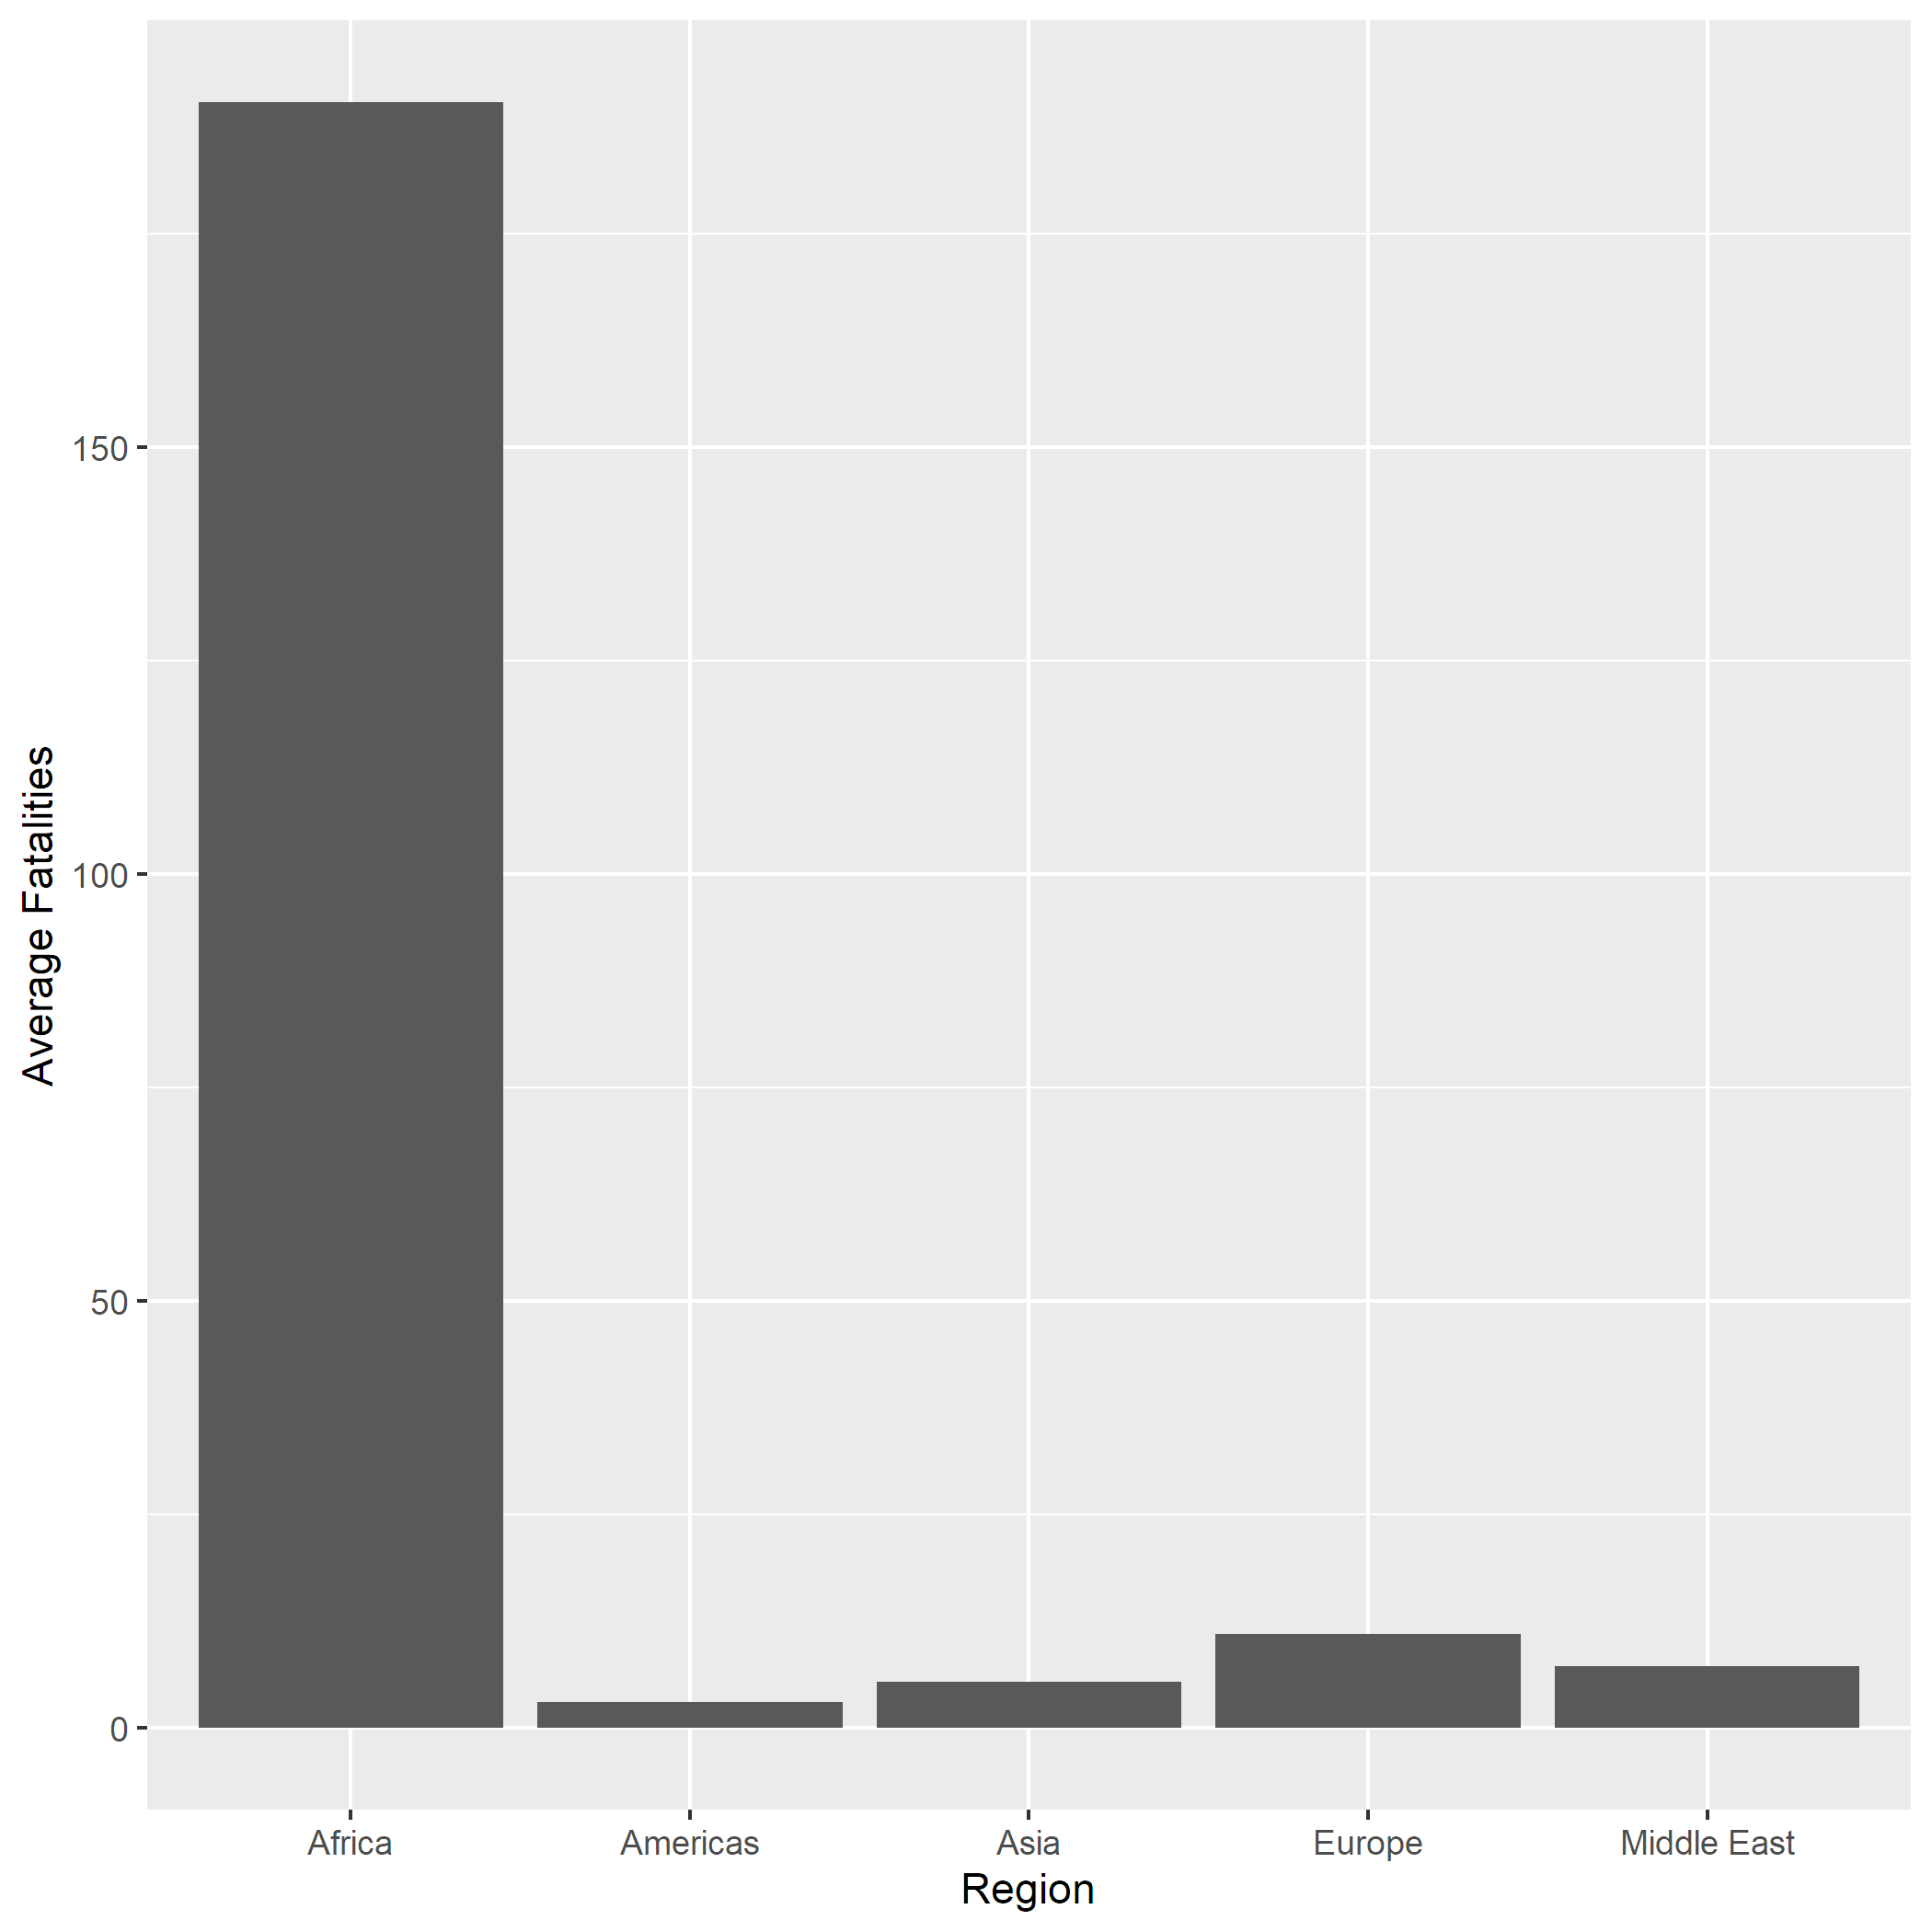
\includegraphics[scale=.8]{fig1_avgfatplot}
  \caption{Average Fatalities Per Incident By Region}
\end{figure} 
\begin{figure}
  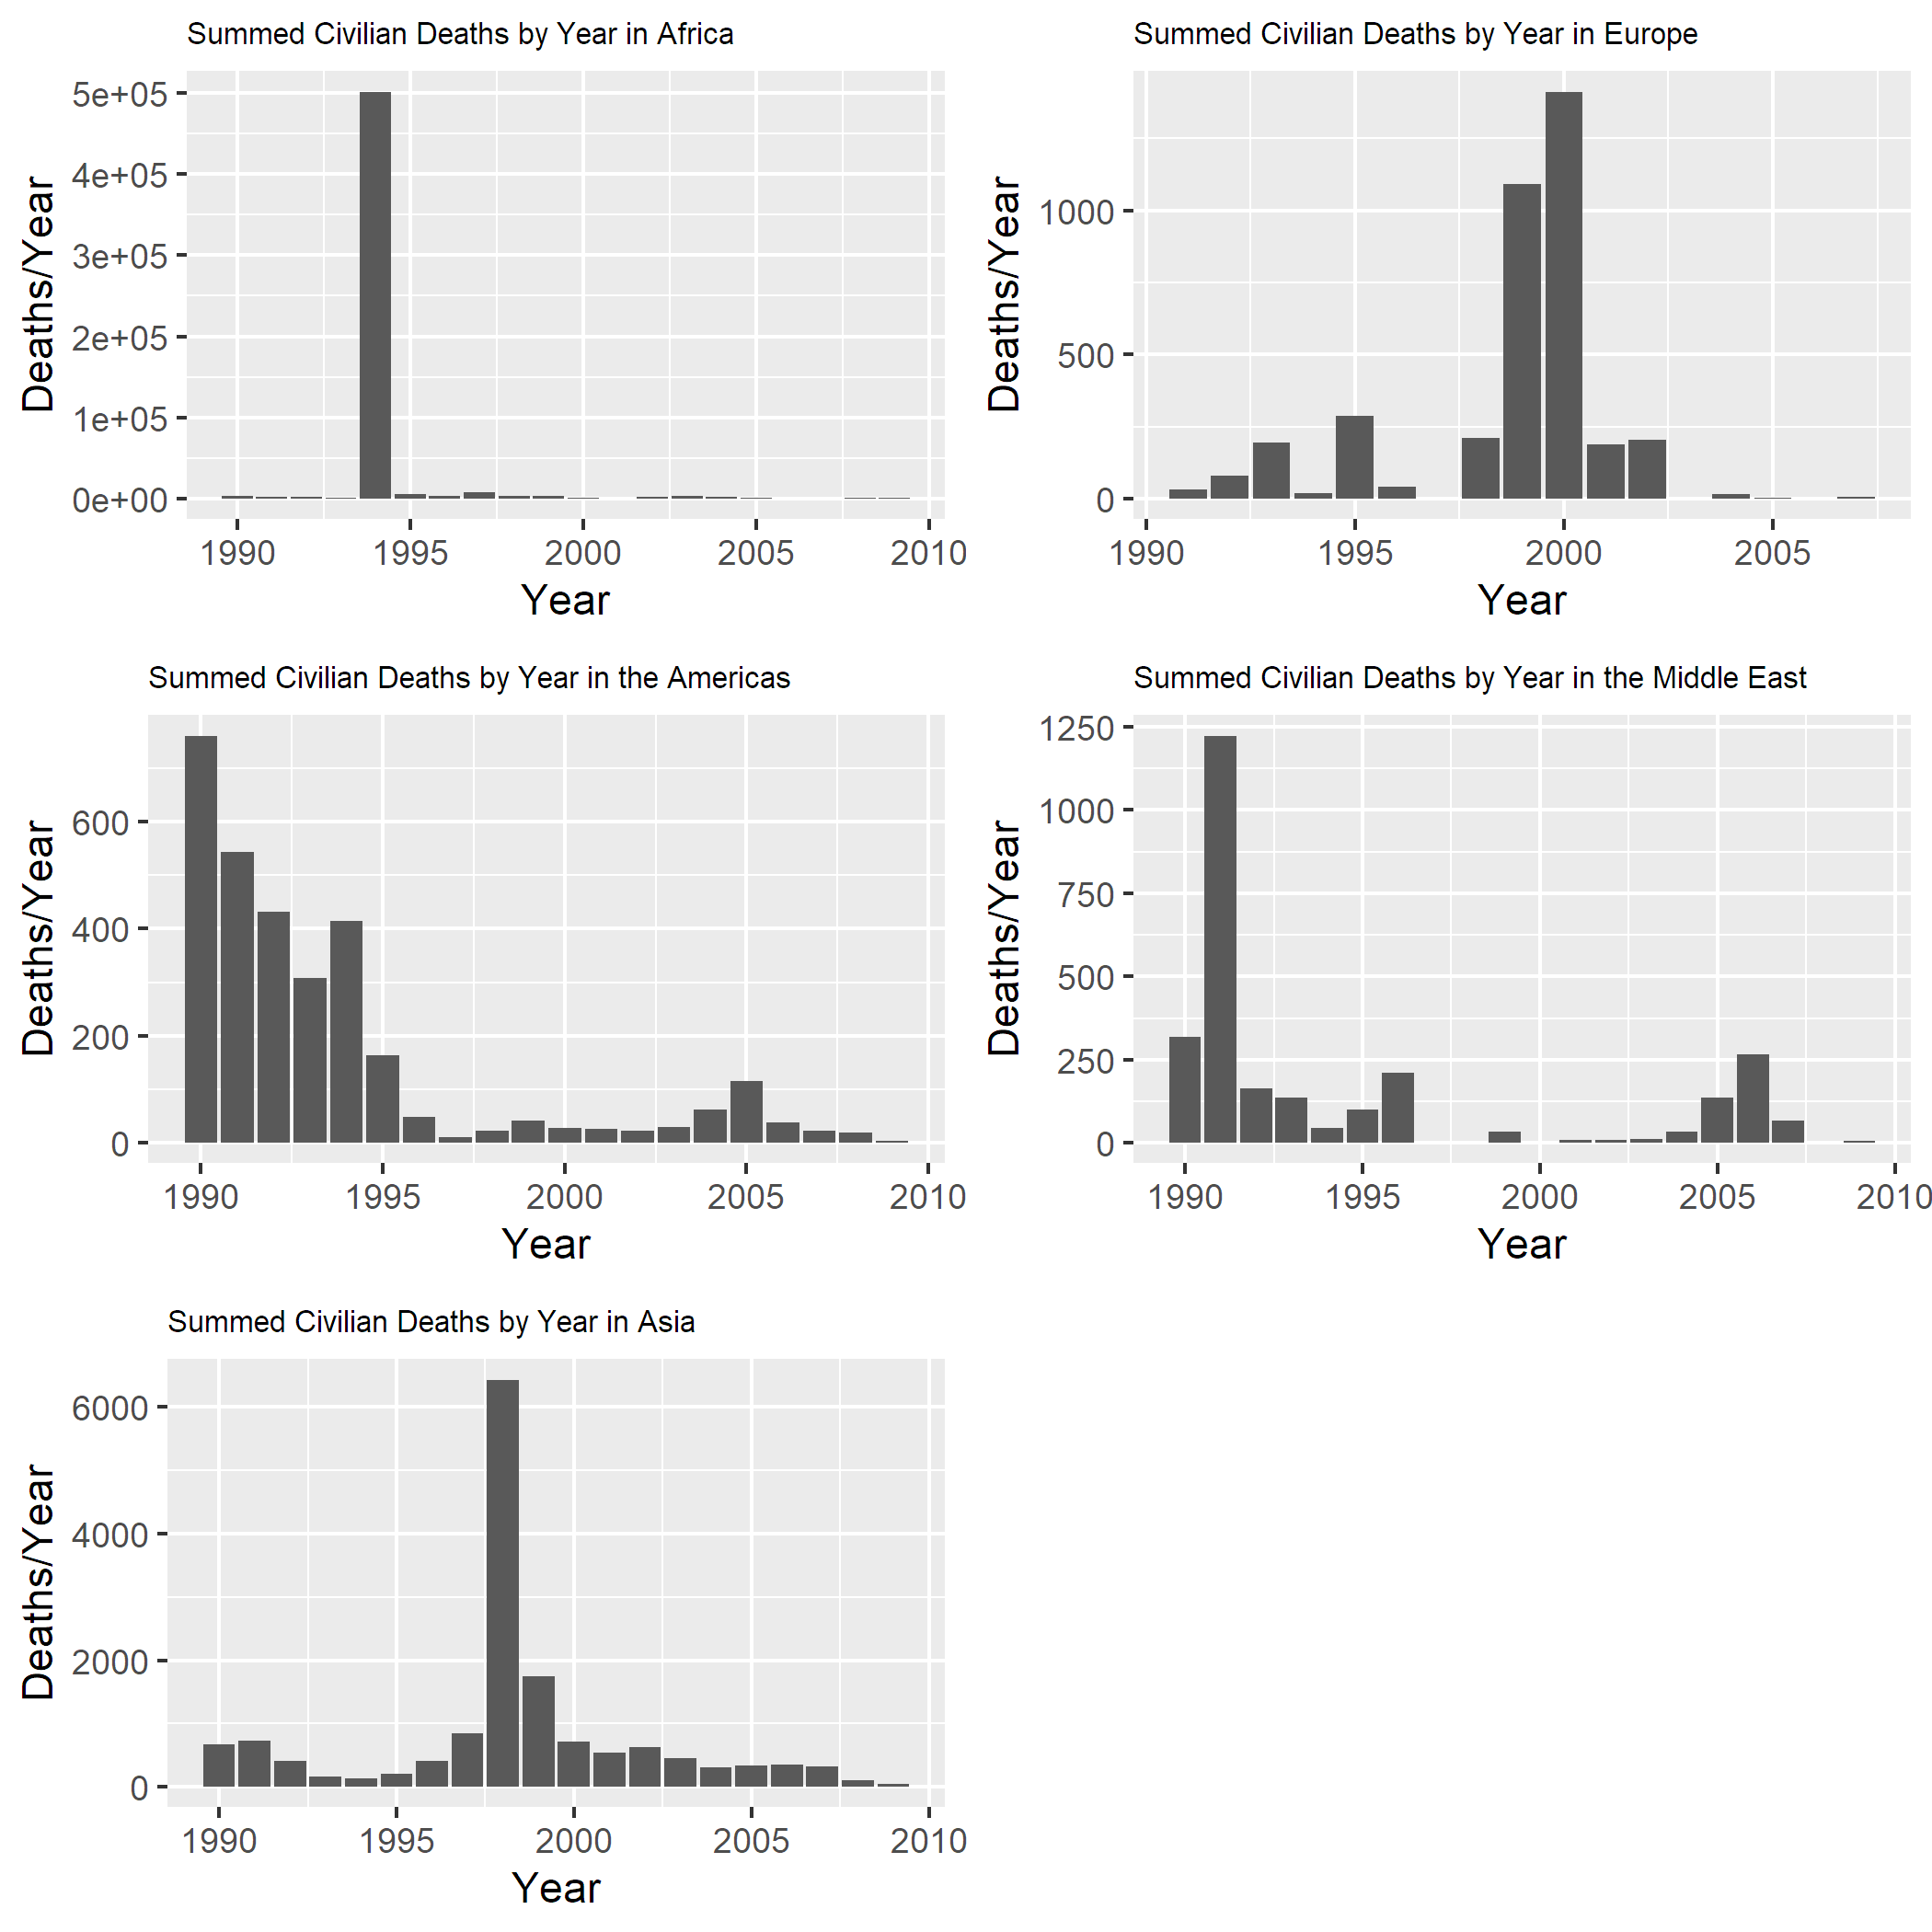
\includegraphics[scale=.9]{fig2}
  \caption{Summed Deaths by Year by Region}
\end{figure} 

Within the cell-year framework, Figure 3 shows the yearly average number of deaths from GED events per year across all cells in the dataset. While this indicates averages very close to 0, with the exception of the year 1994 (which records several instances of mass killings from the Rwandan Genocide), this average is driven down by a large number of zeros due to a lack of violent events in many cells. To remedy this, Figure 4 shows yearly average civilian deaths, calculated only from cells in which at least one GED event occurred per year. This figure excludes 1994 due to the distortionary effects of the Rwandan Genocide; Figure 4.1, which includes the Rwandan Genocide, is shown in the Appendix. This shows more substantial variation, with the majority of years showing an average of under 50 deaths. Figure 5 shows that, despite these casualty numbers, the total number of PRIO-GRID cells containing at least one event of violence per year is quite low, compared to the total of 64,818 individual cells in my dataset. Finally, Figures 6 and 7 show the average gross cell product and average cell population for the original years in which they were measured, which were 1990, 1995, 2000, and 2005, both of which increase in a roughly linear fashion.  

\begin{figure}
	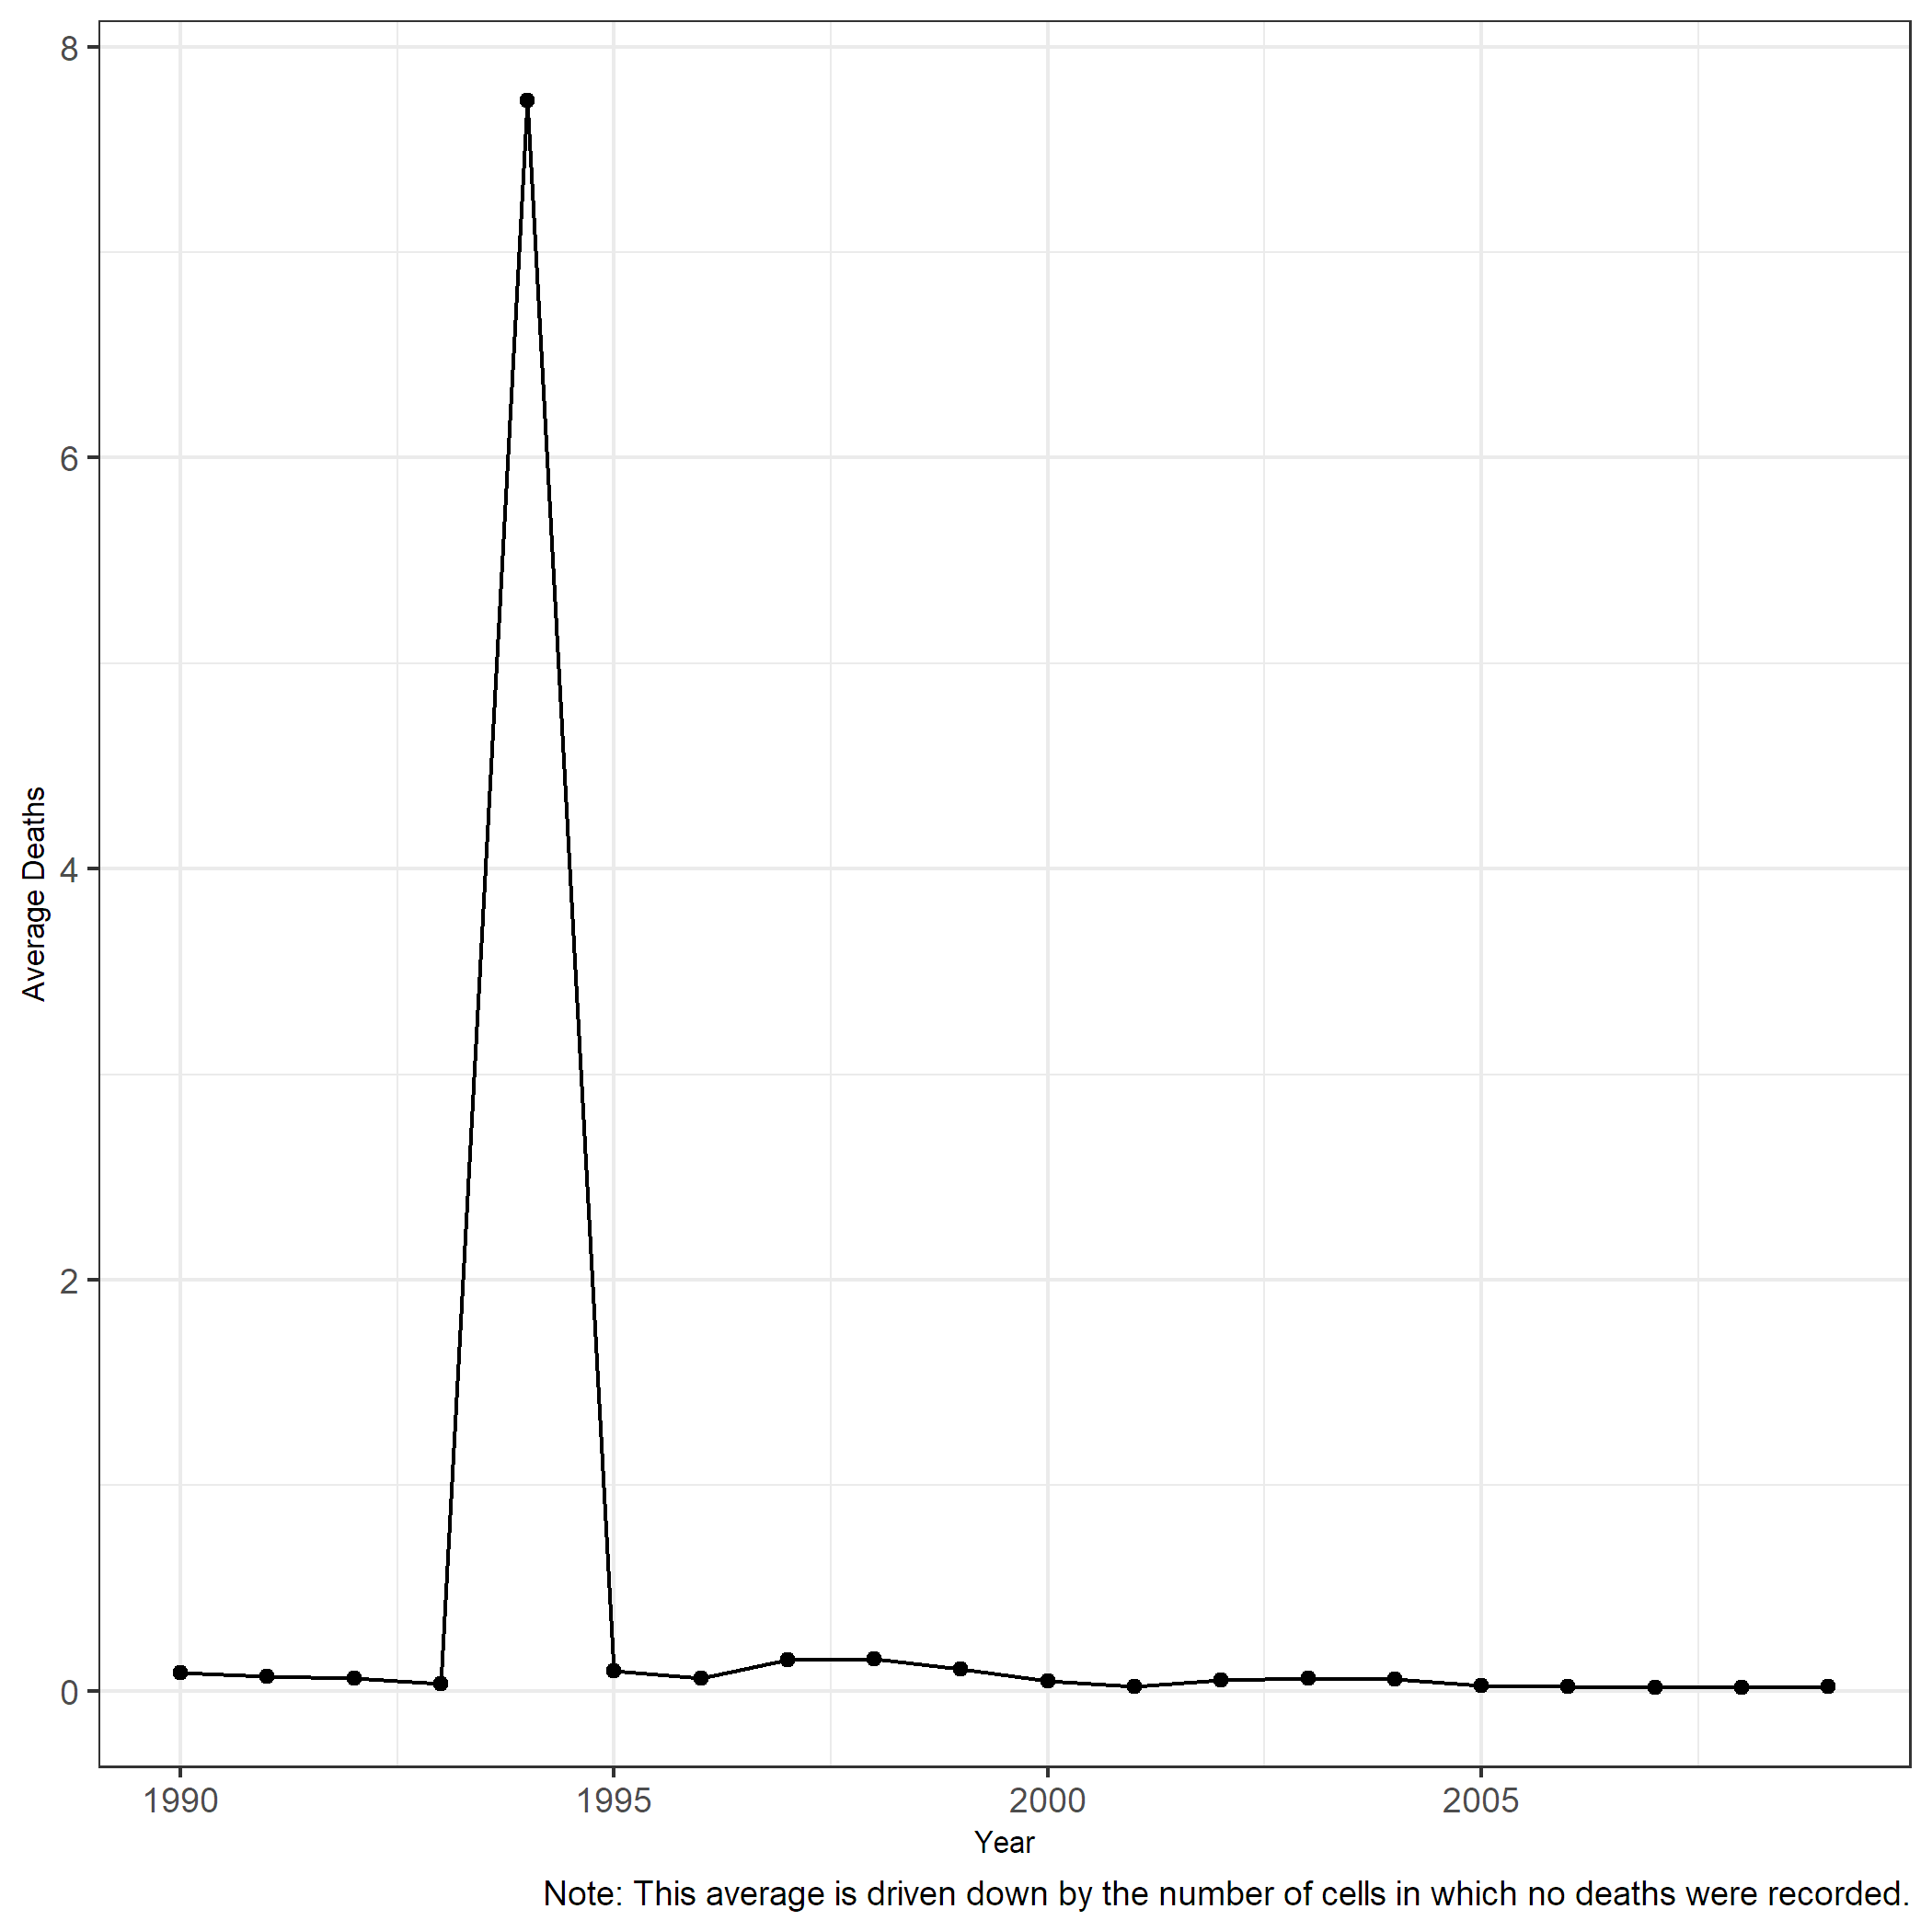
\includegraphics[scale=.7]{fig3}
	\caption{Average of Civilian Deaths Per Year, All Cells}
\end{figure} 
\begin{figure}
	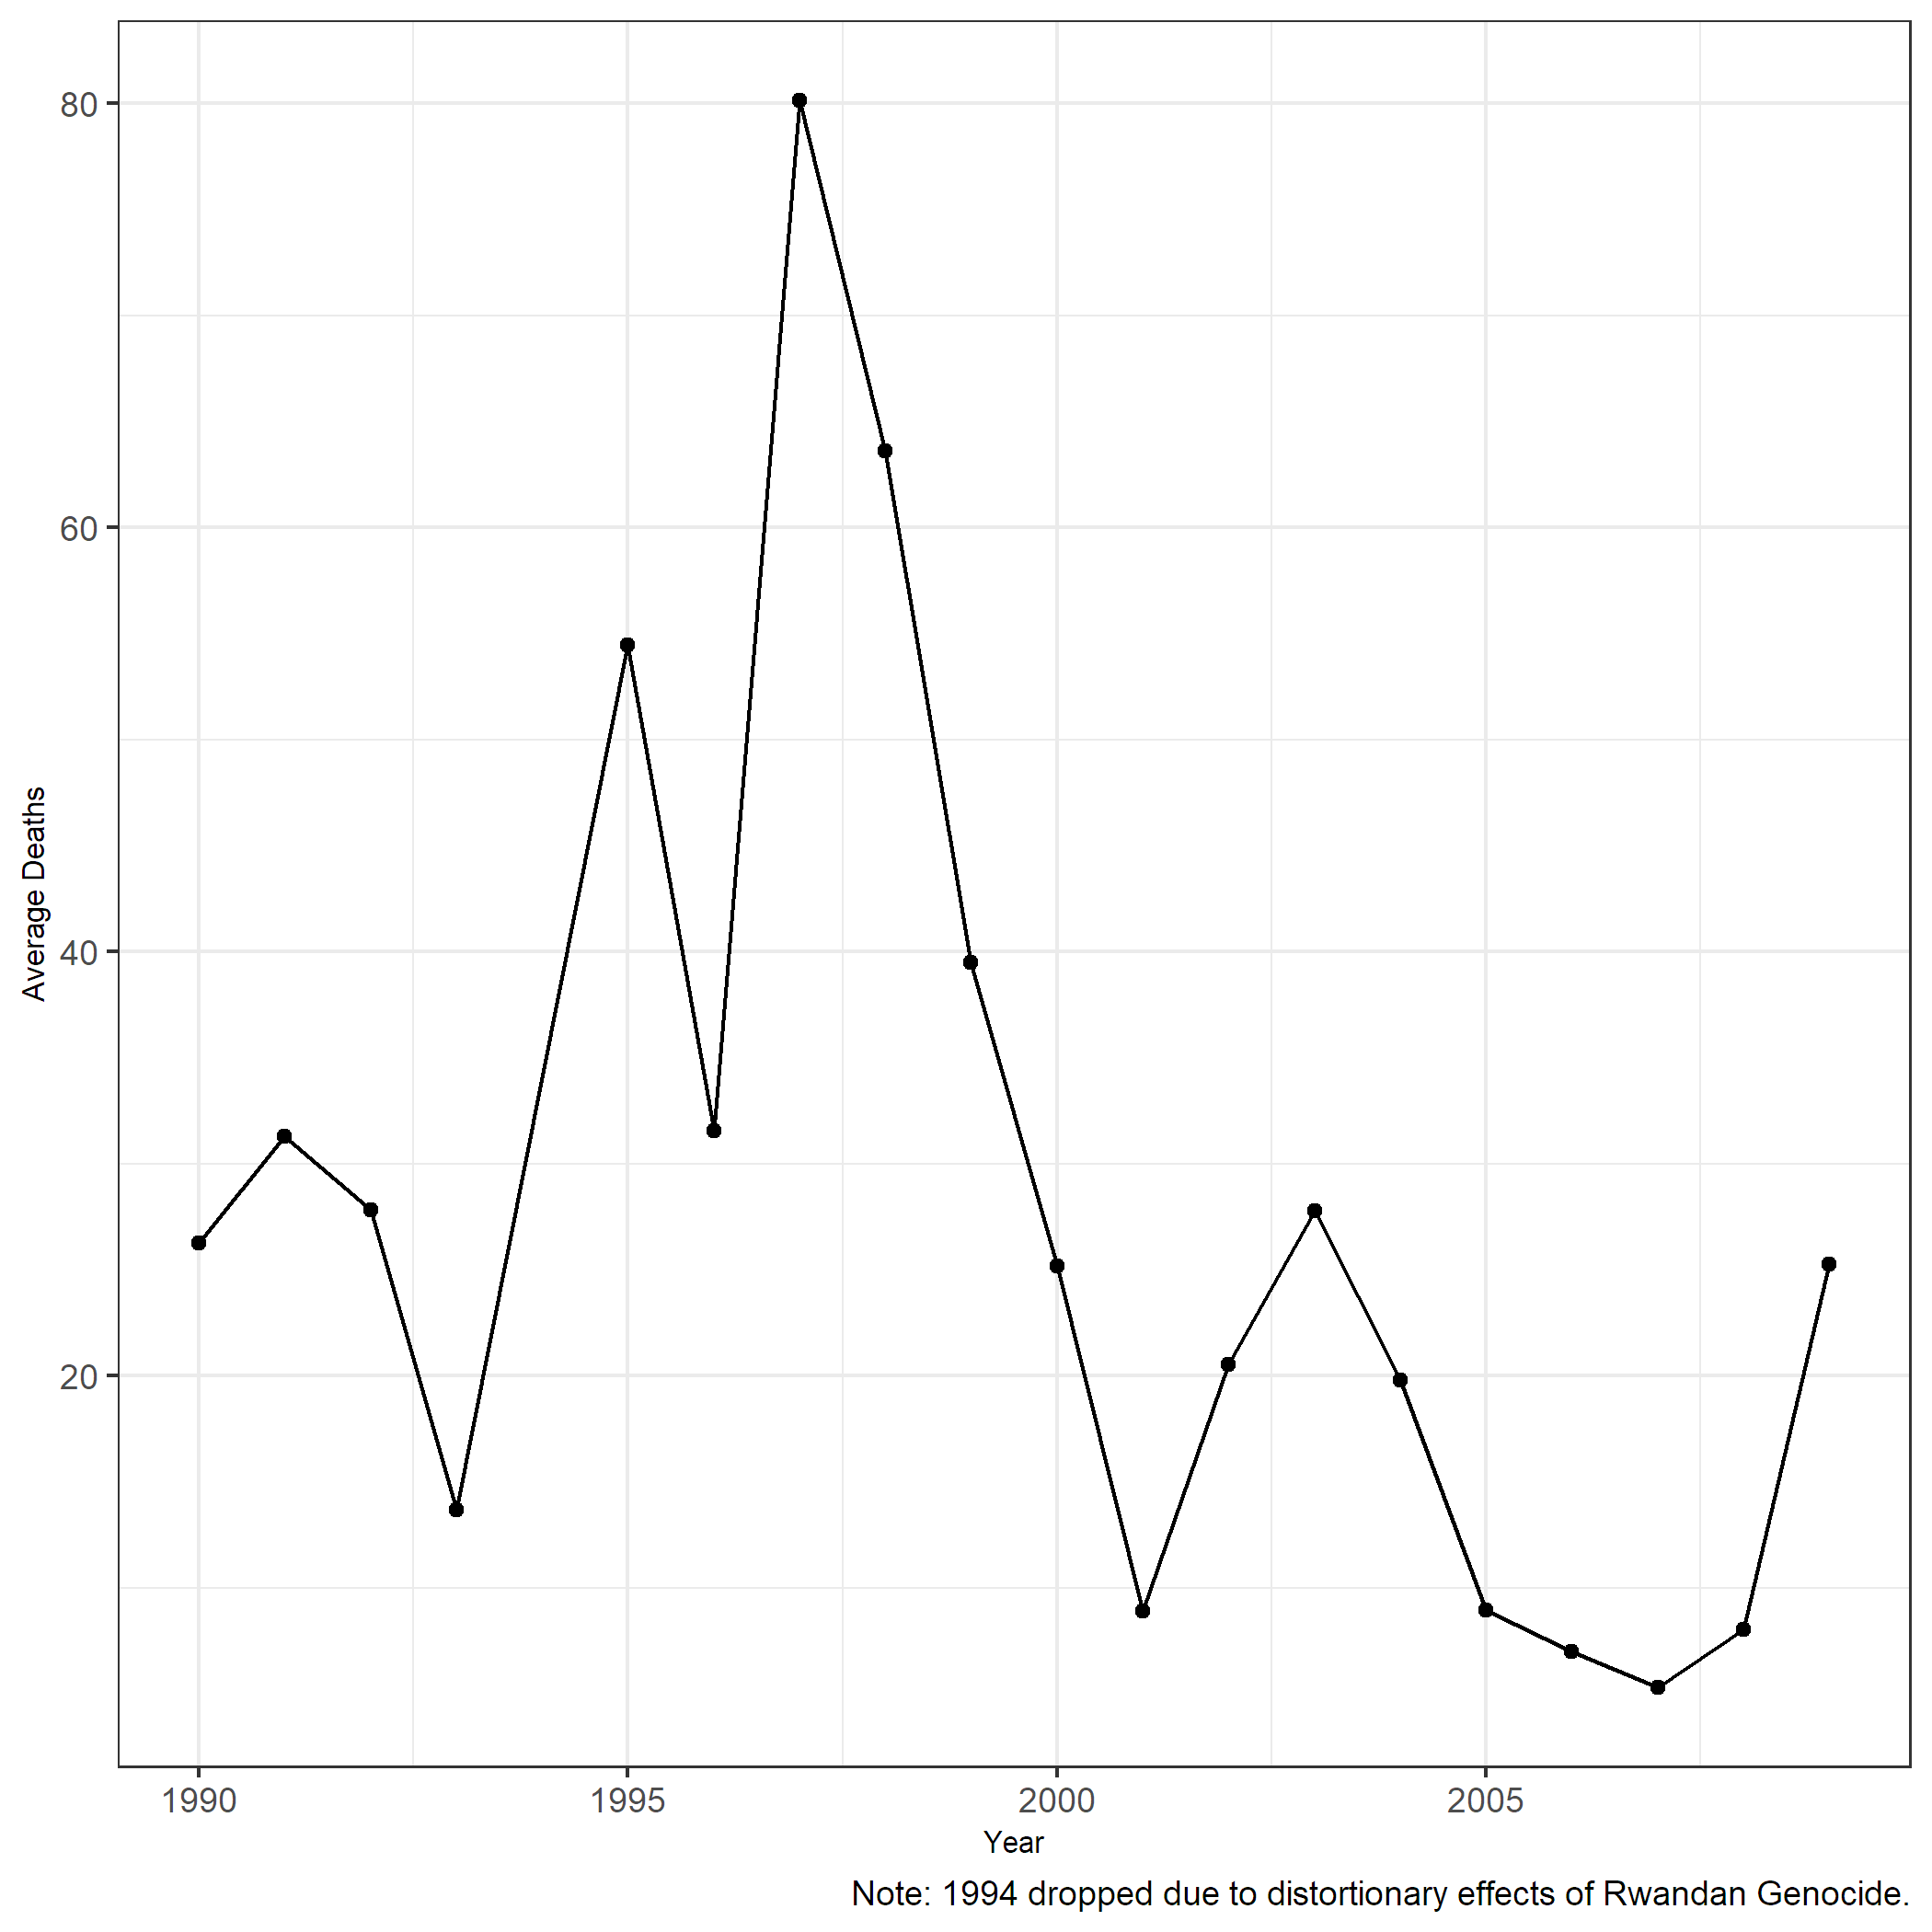
\includegraphics[scale=.7]{fig4}
	\caption{Average of Civilian Deaths Per Year in Cells with GED Violence}
\end{figure} 
\begin{figure}
	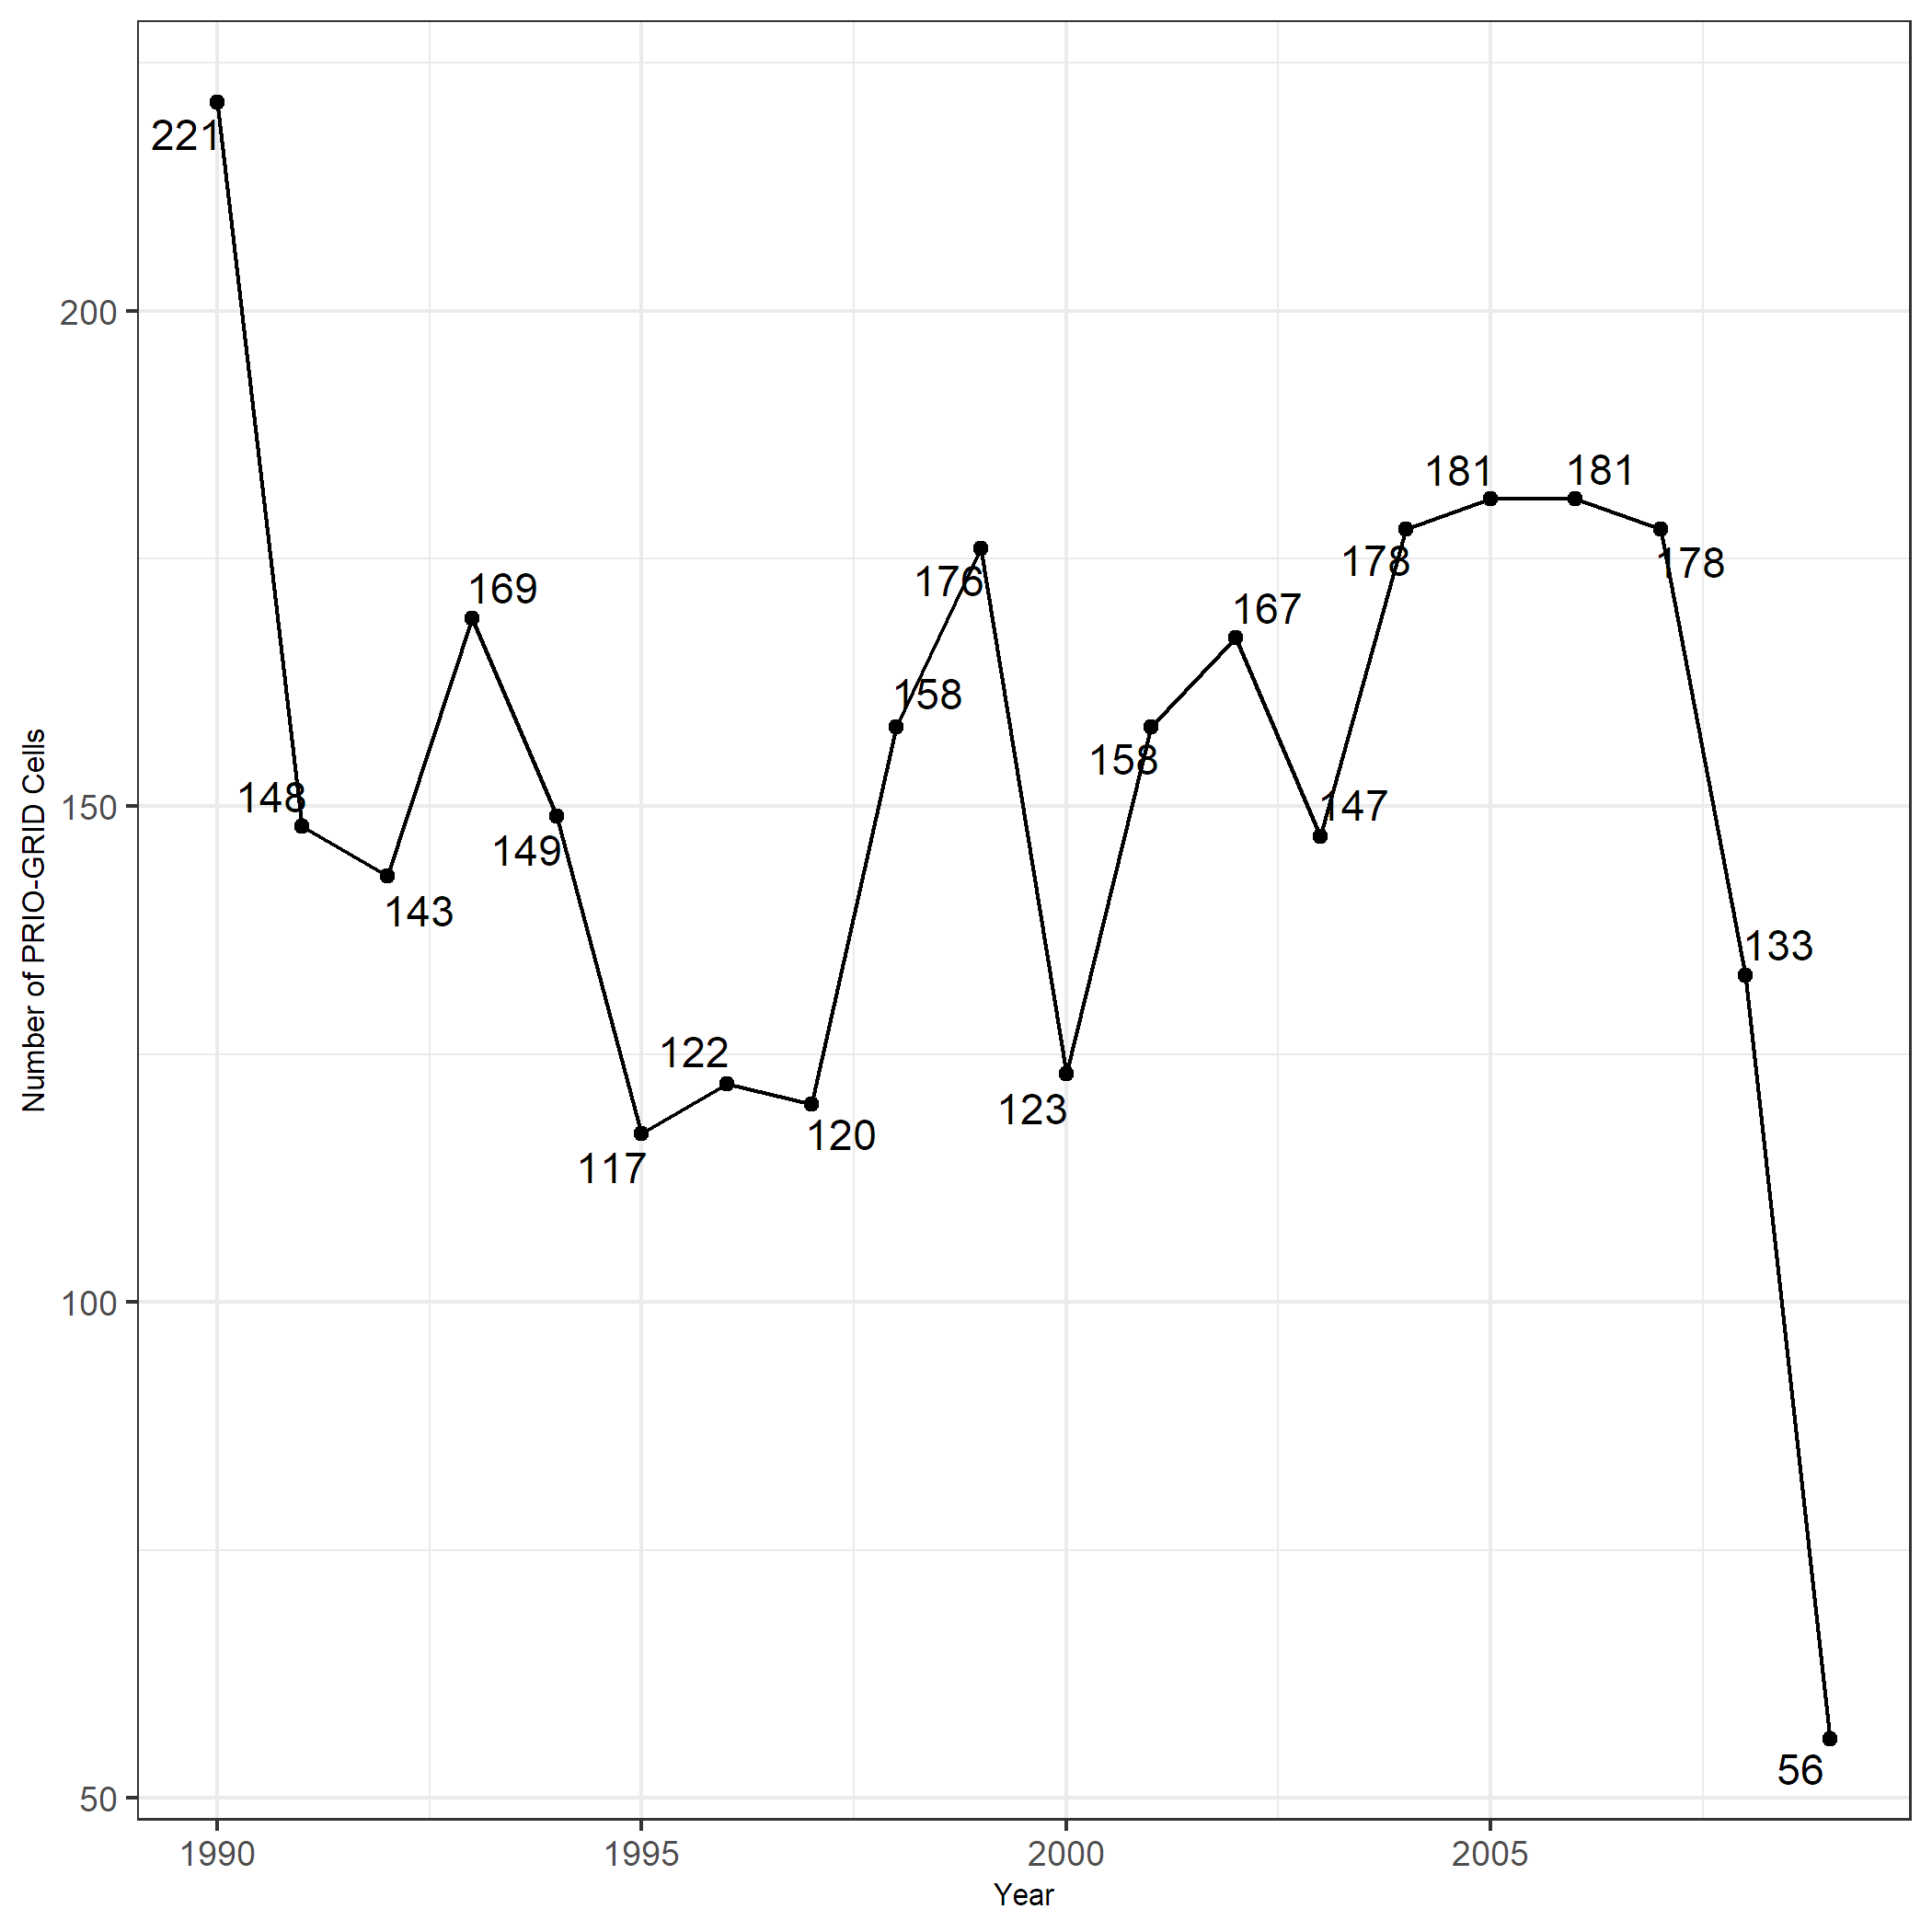
\includegraphics[scale=.7]{fig5}
	\caption{Yearly Counts of Cells with At Least One GED Event}
\end{figure} 
\begin{figure}
	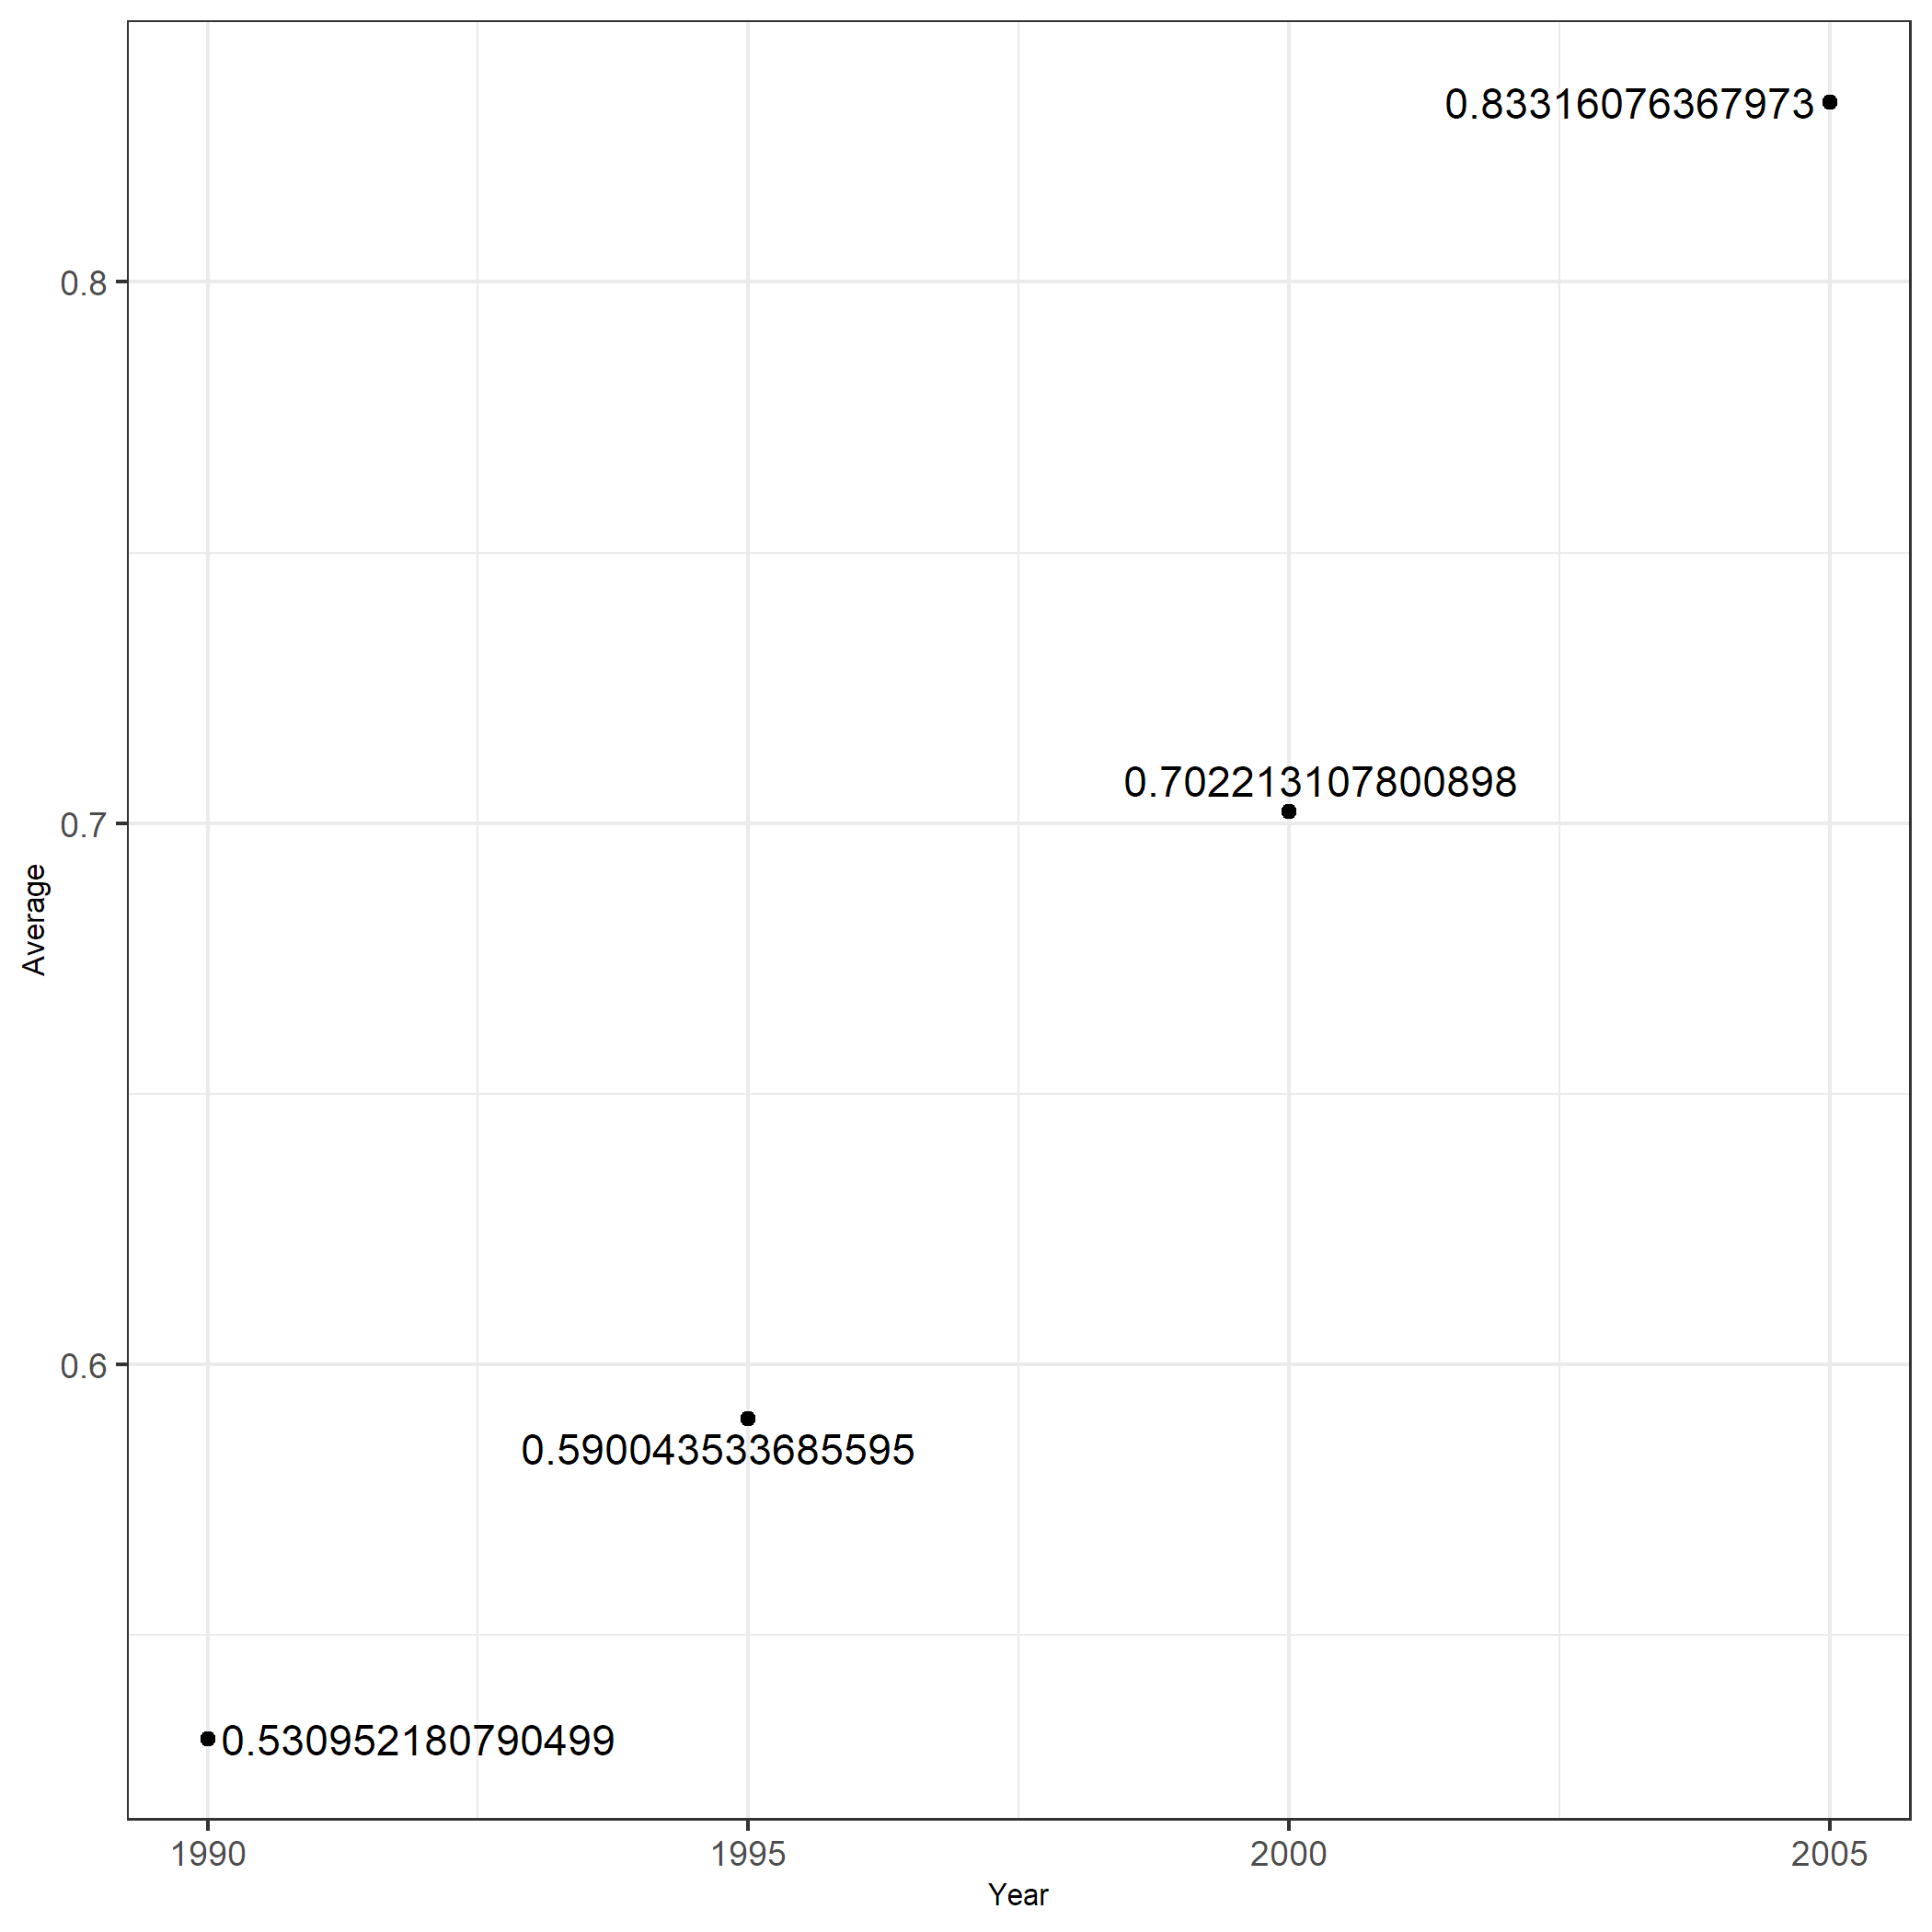
\includegraphics[scale=.7]{fig6}
	\caption{Average Gross Cell Product for Years Measured}
\end{figure} 
\begin{figure}
	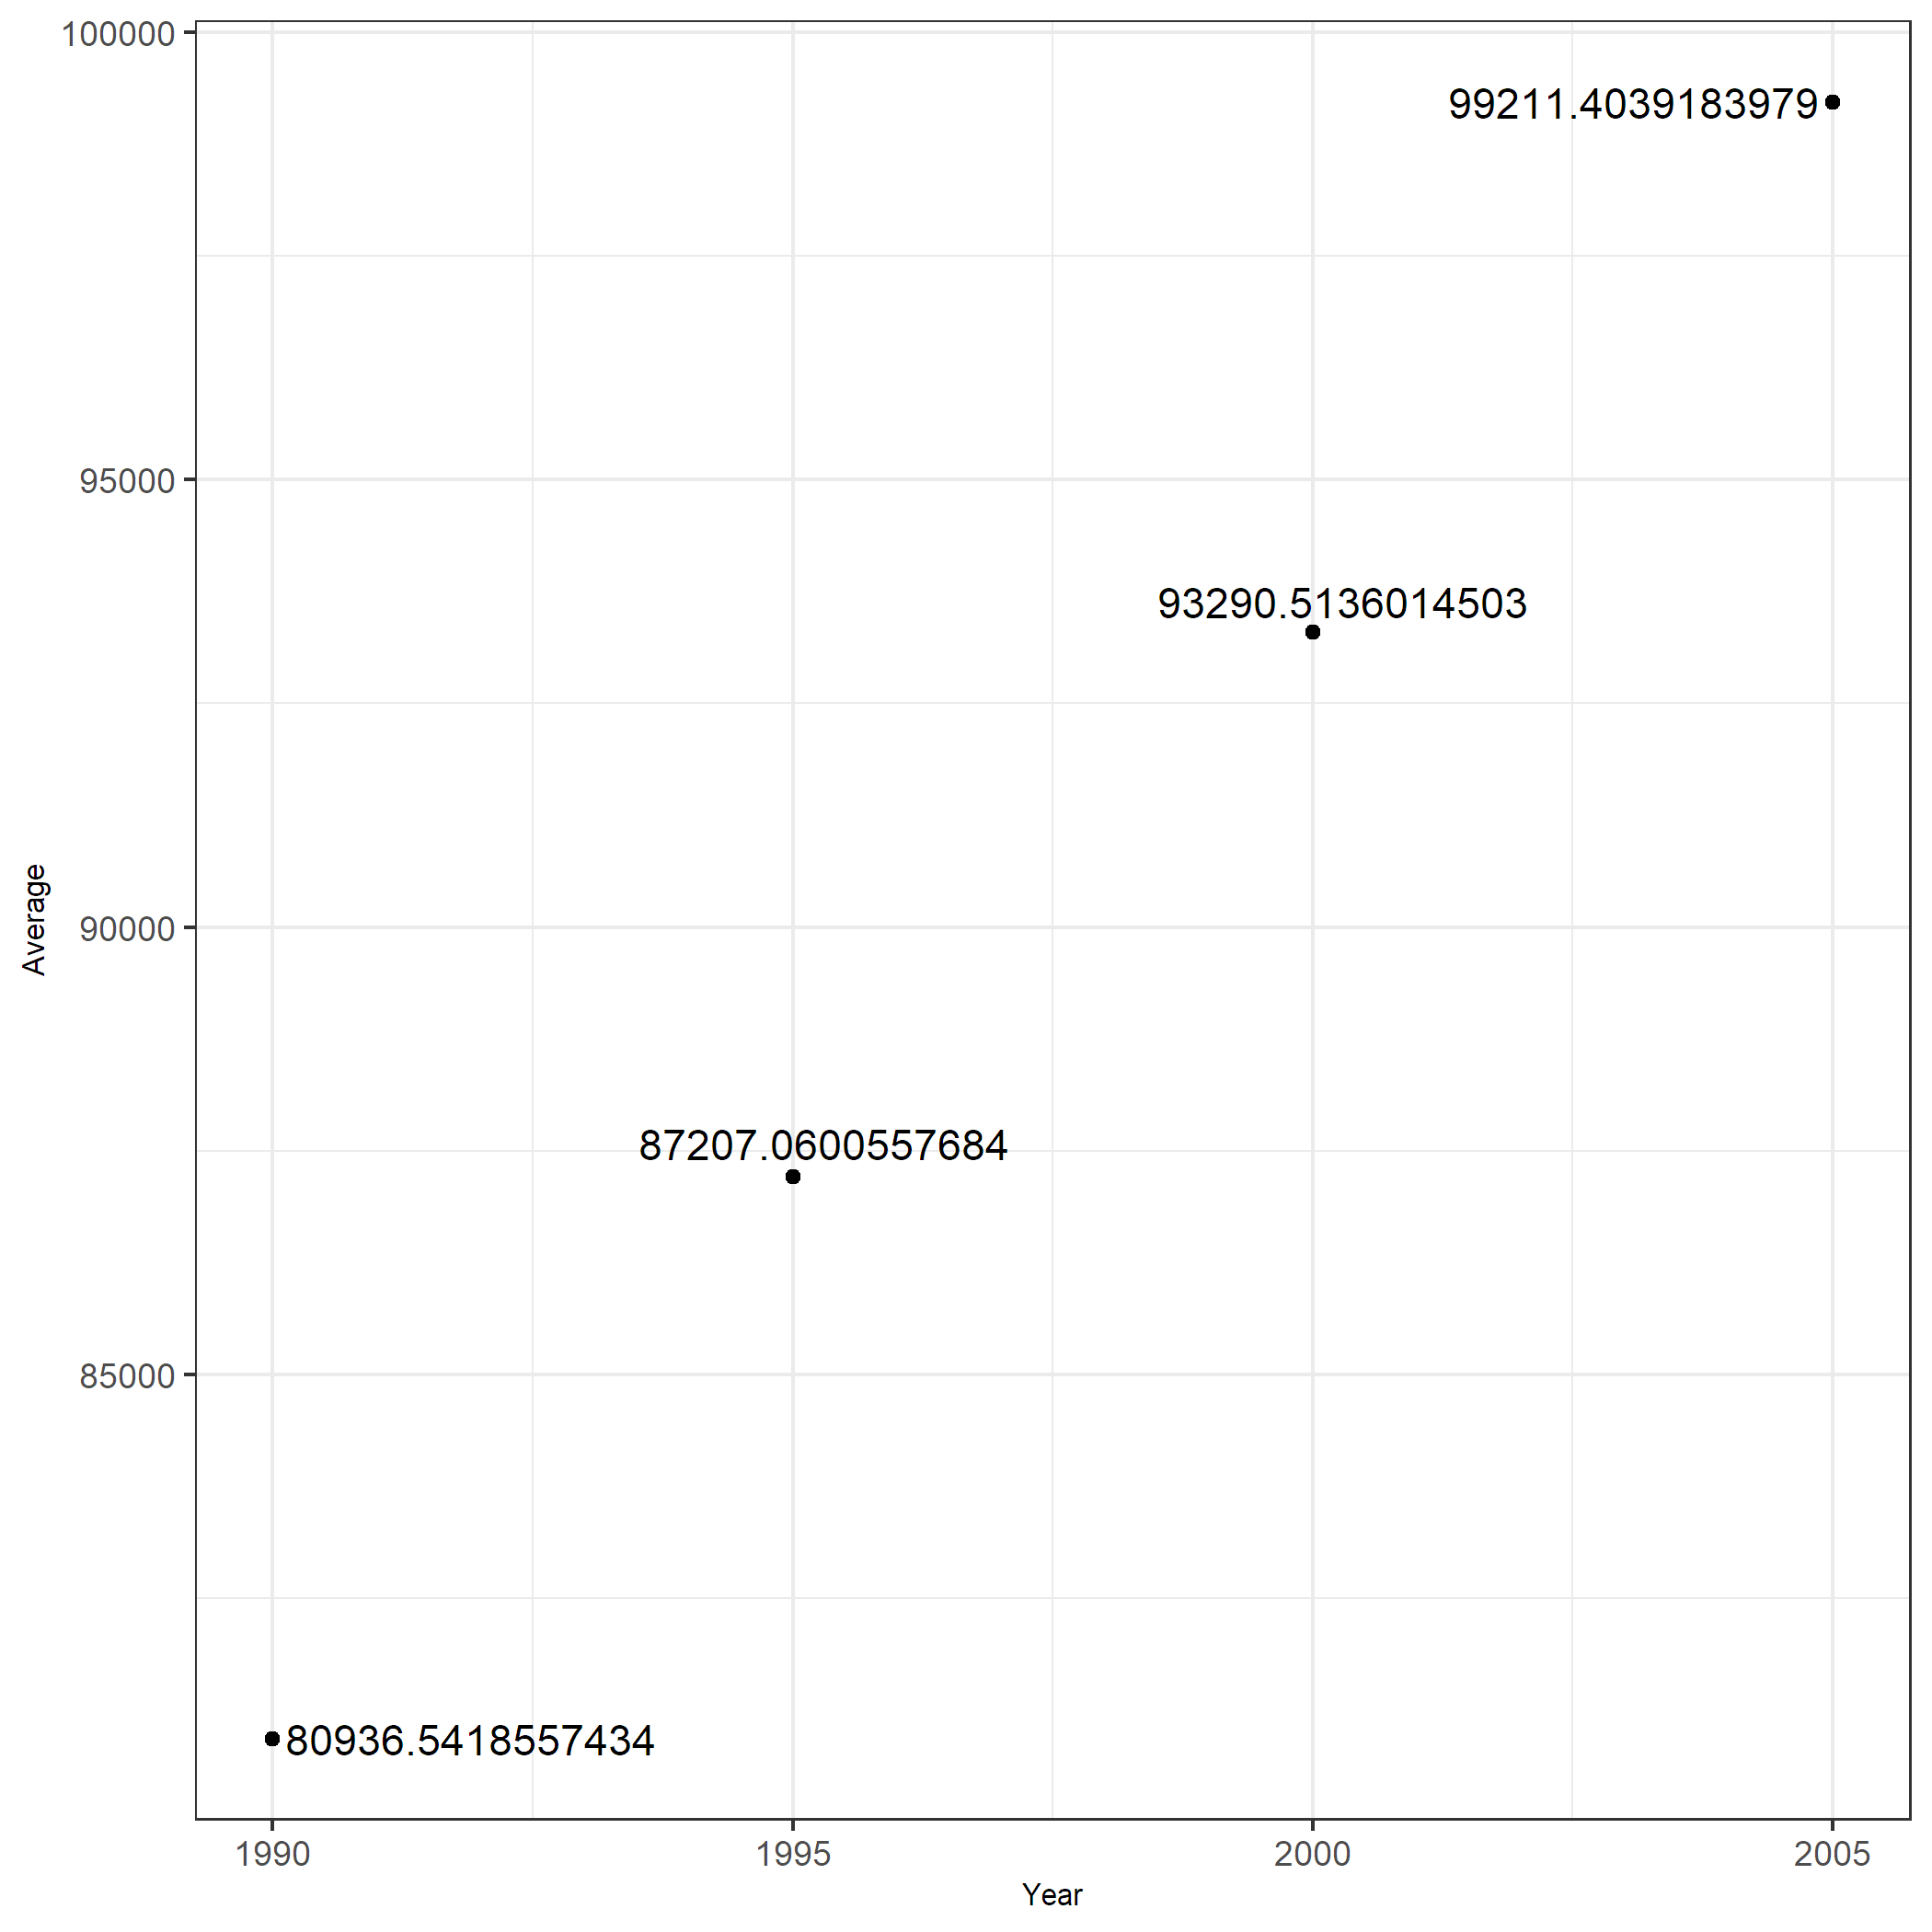
\includegraphics[scale=.7]{fig7}
	\caption{Average Cell Population for Years Measured}
\end{figure} 

\subsection*{Results: Logit Model}
\addcontentsline{toc}{subsection}{Results: Logit Model}
I test my hypotheses using a logit model. The dependent variable of the logit model is a binary indicator of whether an incident of repressive violence occurred within a given grid cell-year. I operationalize the presence of easy- or hard-to-extract resources through binary variables for the presence of lootable diamond and oil deposits, respectively, within a given grid cell for a given year. These enable me to test both of my hypotheses. If the presence of resources increases the probability of an incident of state repression, this will serve as support for my first hypothesis; thus, the first hypothesis will be supported if these variables have positive and significant effects on the probability of repressive violence. By contrast, the second hypothesis will be supported if the effect of easy-to-extract resources on the probability of violence is positive and greater than the effect of hard-to-extract resources on that same probability of violence. This model also includes several control variables. The first is a control for whether the cell-year was experiencing any active conflict, as defined by the UCDP \cite{Stina19}, in order to control for the confounding effects of preexisting high levels of violence within a cell-year, such as those due to civil war. The second and third are standard controls for the gross cell product per cell-year and the cell’s population per cell-year, as described in the previous section. Finally, there is a control for the year.

\begin{table}[h] \centering 
	\caption{Logit Model 1 Regression Results} 
	\label{} 
	\begin{tabular}{@{\extracolsep{5pt}}lc} 
		\\[-1.8ex]\hline 
		\hline \\[-1.8ex] 
		& \multicolumn{1}{c}{\textit{Dependent variable:}} \\ 
		\cline{2-2} 
		\\[-1.8ex] & Probability of Violence \\ 
		\hline \\[-1.8ex] 
		Active Conflict Dummy & 6.310$^{***}$ \\ 
		& (0.053) \\ 
		Lootable Diamond Dummy & 0.803$^{***}$ \\ 
		& (0.155) \\ 
		Petroleum Dummy & $-$0.101 \\ 
		& (0.063) \\ 
		Gross Cell Product & $-$0.016$^{***}$ \\ 
		& (0.006) \\ 
		Cell Population & 0.00000$^{***}$ \\ 
		& (0.00000) \\ 
		Year & $-$0.024$^{***}$ \\ 
		& (0.003) \\ 
		Constant & 40.108$^{***}$ \\ 
		& (6.934) \\ 
		\hline \\[-1.8ex] 
		Observations & 1,296,360 \\ 
		Log Likelihood & $-$10,768.490 \\ 
		Akaike Inf. Crit. & 21,550.980 \\ 
		\hline 
		\hline \\[-1.8ex] 
		\textit{Note:}  & \multicolumn{1}{r}{$^{*}$p$<$0.1; $^{**}$p$<$0.05; $^{***}$p$<$0.01} \\ 
	\end{tabular} 
\end{table}

\subsection*{Analysis: Logit Model}
\addcontentsline{toc}{subsection}{Analysis: Logit Model}
As shown in Table 1, all variables are significant except for the petroleum dummy variable. Additionally, the indicator variable for the presence of diamonds is positive, as predicted by my first hypothesis. Figure 8 shows the predicted effects of the presence of diamonds on the probability of state repression, using the average case approach and holding all other variables at their modes or means, which were 0 for all of the other binary indicators. This figure shows that the presence of diamonds does have a large, positive impact on the probability of state repression. While the substantive increase in the probability of violence is rather small, this is likely due to the low probability of violence in the dataset in general, as shown above in Figure 5 of the descriptive statistics. Given this overall low probability of violence, this increase in its probability is still substantively meaningful. This ultimately provides support for the first hypothesis, as the presence of at least one of type of resource does increase the probability of repressive violence by a meaningful amount, relative to the overall probability of violence in the data. 

\begin{figure}
	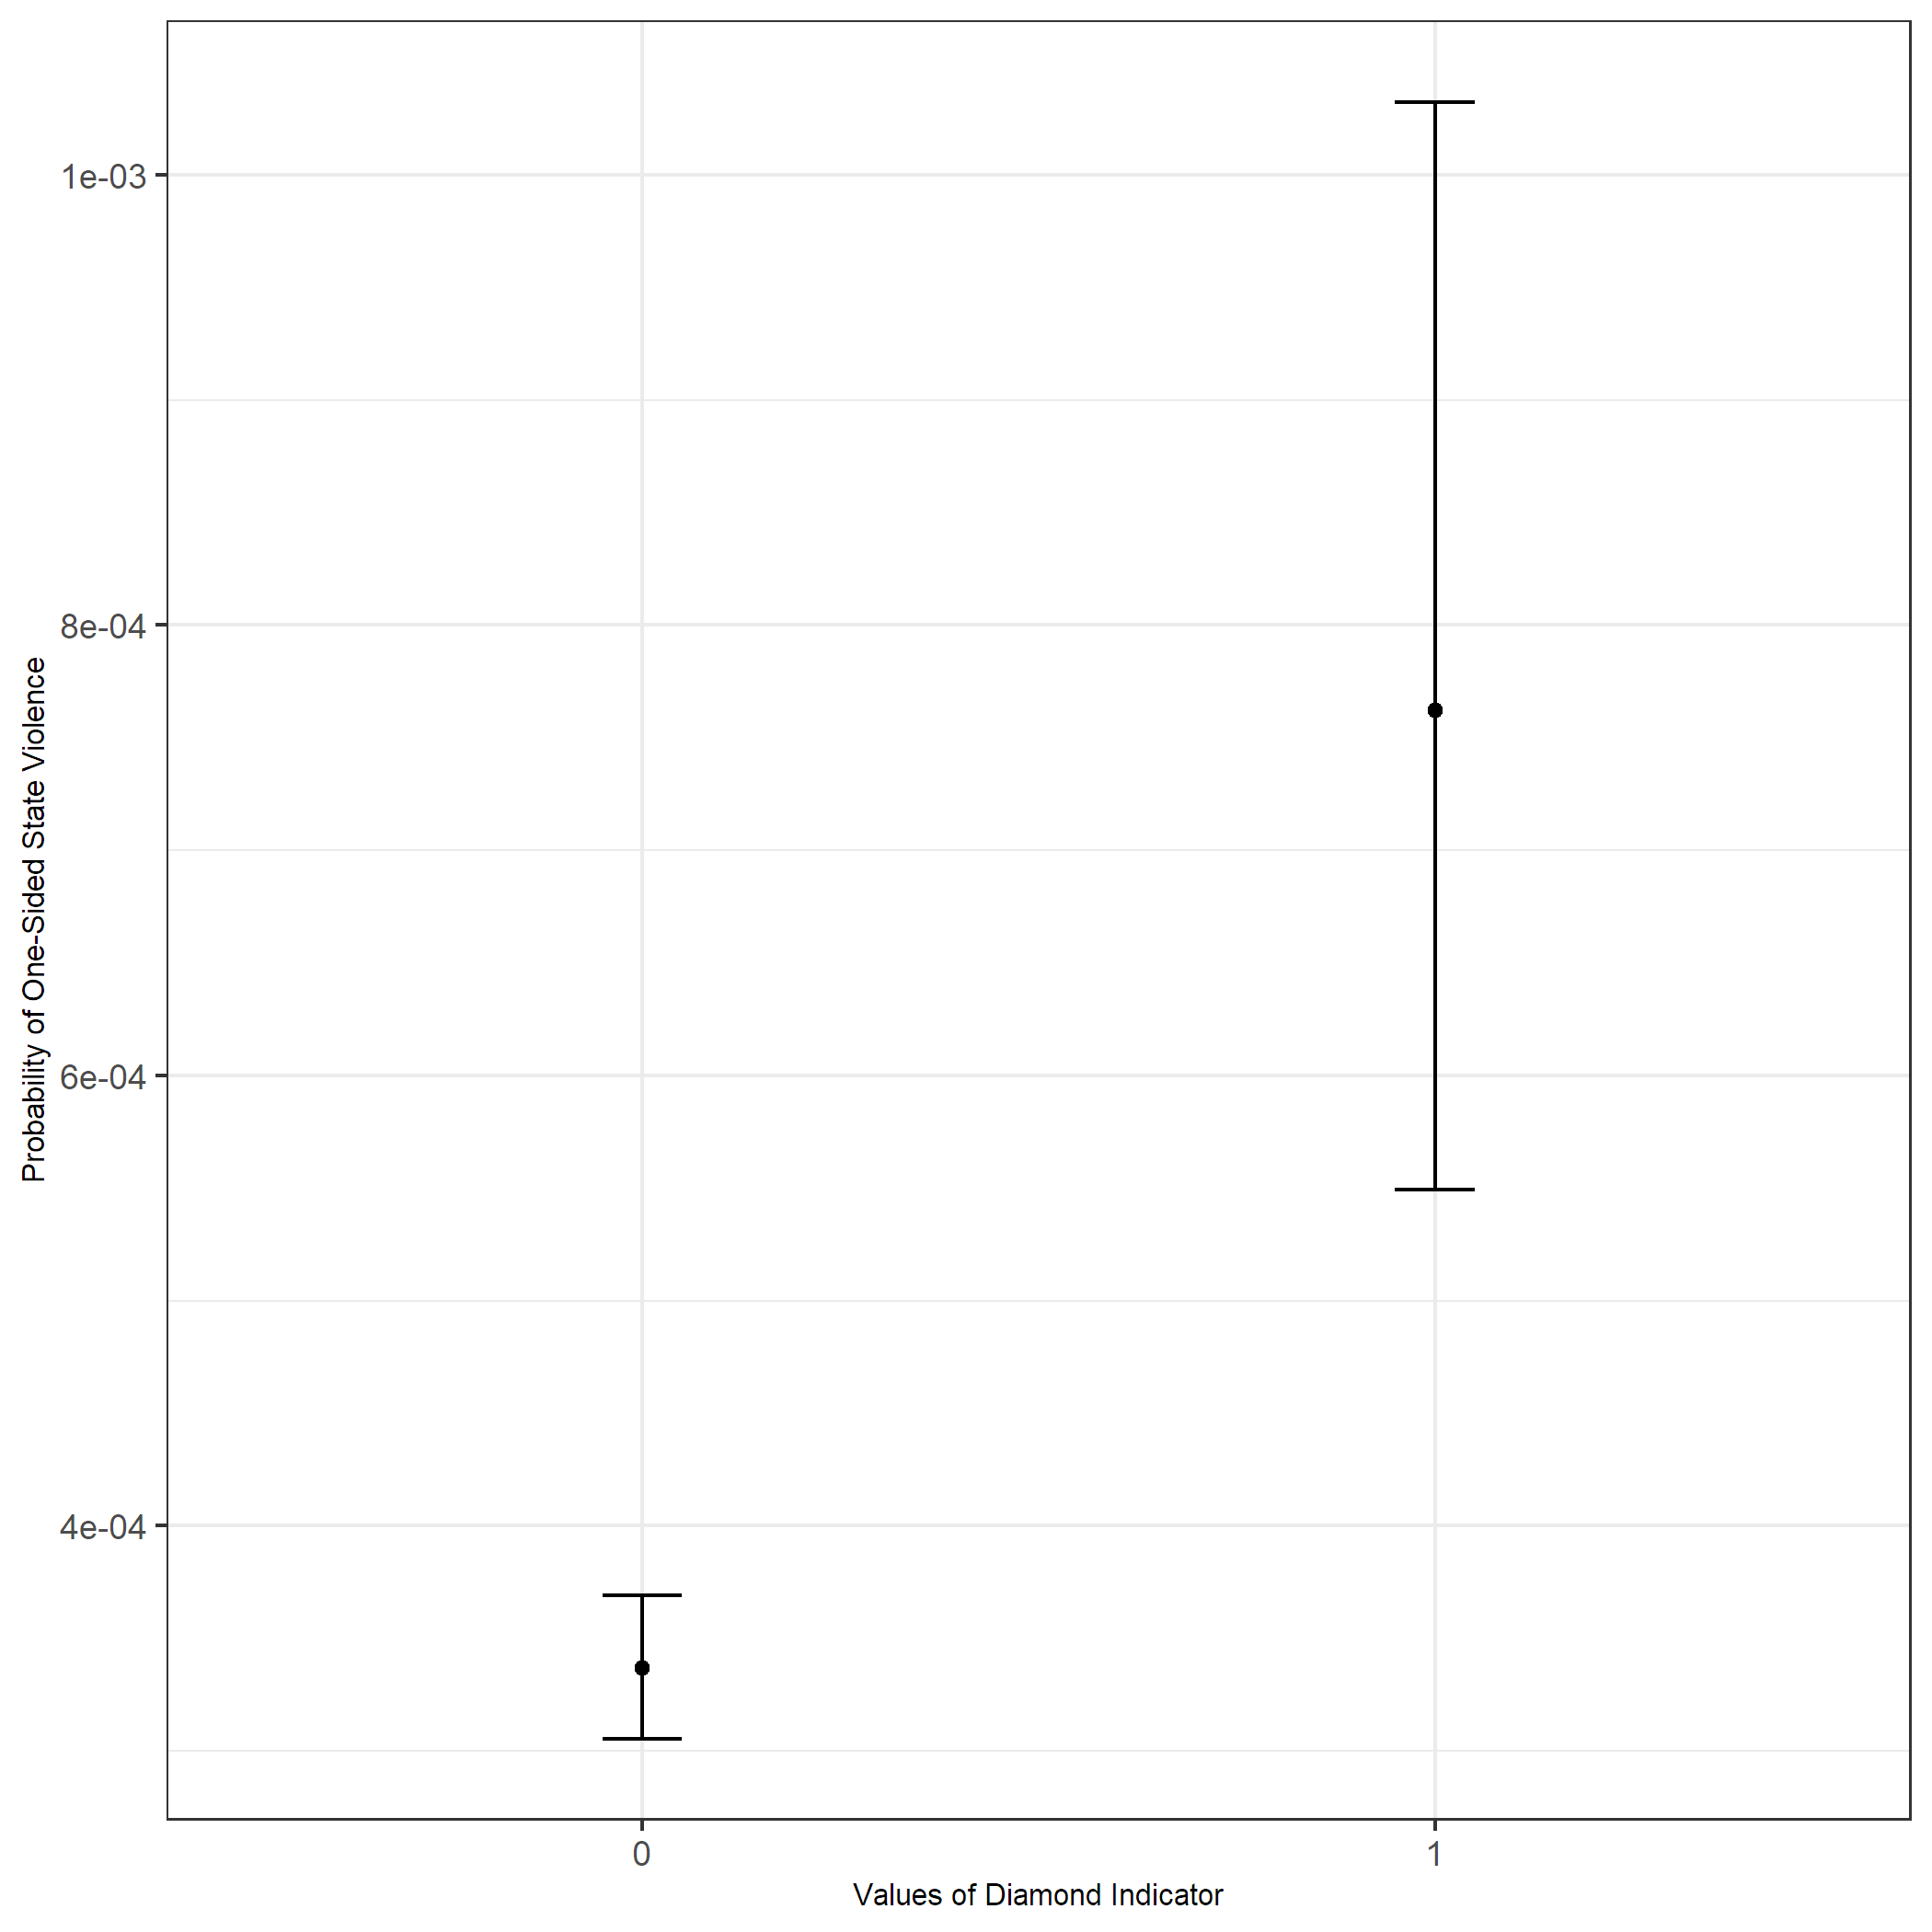
\includegraphics[scale=.8]{fig8}
	\caption{Predicted Probability of State Violence using Average Case Approach, with 95\% CIs}
\end{figure} 

Due to the lack of significance at the $p=.05$ level for the petroleum dummy variable, this result does not fully support the second hypothesis. While the positive and significant effect of lootable diamonds on the probability of state repression is as predicted, the non-significant effect of petroleum on the probability of state repression is not. While this finding shows that the presence of lootable resources does increase the probability of state repression in the vicinity of those resources, which provides support for part of the theory, this failure to find a significant effect for non-lootable resources indicates that the mechanisms proposed in the theory may be more limited in their scope than initially assumed. 

\newpage
\vspace*{25pt}
\section*{\normalfont \hfill DISCUSSION AND CONCLUSION \hfill}
\addcontentsline{toc}{chapter}{DISCUSSION AND CONCLUSION}
These results provide some support for the theory. The logit model supported the first hypothesis, due to the strong positive effect of the presence of diamonds on the probability of state repression, but failed to fully support the second hypothesis. While the lack of more conclusive support for the theory is disappointing, there are some theoretical and methodological criticisms to consider before coming to a final verdict on this design. The first is the question of whether a standard logit model is actually the best model for the count data used to test the second hypothesis. The small absolute probabilities, due to the high number of zeros in the data, raise the question of whether a variant that accounts for those zeros is called for, such as a zero-inflated logit. A second potential criticism, and one that cannot be fixed by changes to the model itself, is that the unit of analysis may not be fine enough to pick up on the effects of resources. Given that PRIO-GRID cells are approximately 55 by 55 kilometers, these cells may simply be too large an area, leading to a failure to detect the true directions or significance of effects. A third potential criticism, this time focusing on the data, is the need to expand the range and coverage of the resource data, as the PRIO resource data only covers onshore petroleum deposits discovered through 2003 \cite{TRL7} and diamond deposits discovered to 2005 \cite{Gilmorecode}, and the PRIO-GRID resource coding draws from those two datasets. Ideally, future analyses could also incorporate more than just these two archetypal resources. 

In spite of these issues, this analysis can still serve as a useful starting point for future research. One way in which it can do this is by motivating further refinement of the theory, to account for these findings. The lack of significance for the petroleum indicator in the logit model, despite the strong significance for the diamonds indicator, may indicate that different mechanisms are operating for petroleum resources than for diamond resources—more generally, that resources requiring external investment differ in some meaningful way from those that do not. While these precise mechanisms are unclear, future investigations could test this theory for other types of resources, such as precious metals, to see if they return similar results. Another avenue of investigation could be the use of case studies to uncover refinements to the causal mechanisms.

This is not the only potential theoretical development to be suggested by these results. An alternative direction could involve the strategic decision-making process at the firm level. While firm preferences are not extensively theorized here, this may benefit from additional specification. One possibility for expansion involves examining whether firms have preferences over repression—how much do firms pay attention to state behavior, and what are the conditions under which they do so? Such an expanded theory could provide insights not only into the effects of state repression but also potentially into the investment decisions of multinational firms. This could also potentially lead to models of the strategic interactions of the state and multinational corporations. 

Regardless of these potential future developments, however, the partial support for the theory provides an encouraging sign that this research still contributes a novel meaningful relationship between some types of resources and state repression. These results suggest that, once both geography and the need for external investment are accounted for, only easily lootable resources increase the probability of repressive violence by the state. This indicates that the linkage of resources and state violence is conditional, in at least some cases, on the geographic locations of those resources and the absence of requirements for international investment to enable their extraction. In short, both geographic location and the potential need for international investment influence the probability of observing a linkage between resources and state repressive violence. This novel finding ultimately helps to advance knowledge of the relationship between resources and violence, while providing several potential starting points for future work.

\newpage
\section*{\normalfont \hfill APPENDIX \hfill}
\addcontentsline{toc}{chapter}{APPENDIX}



\begin{figure}[h]
	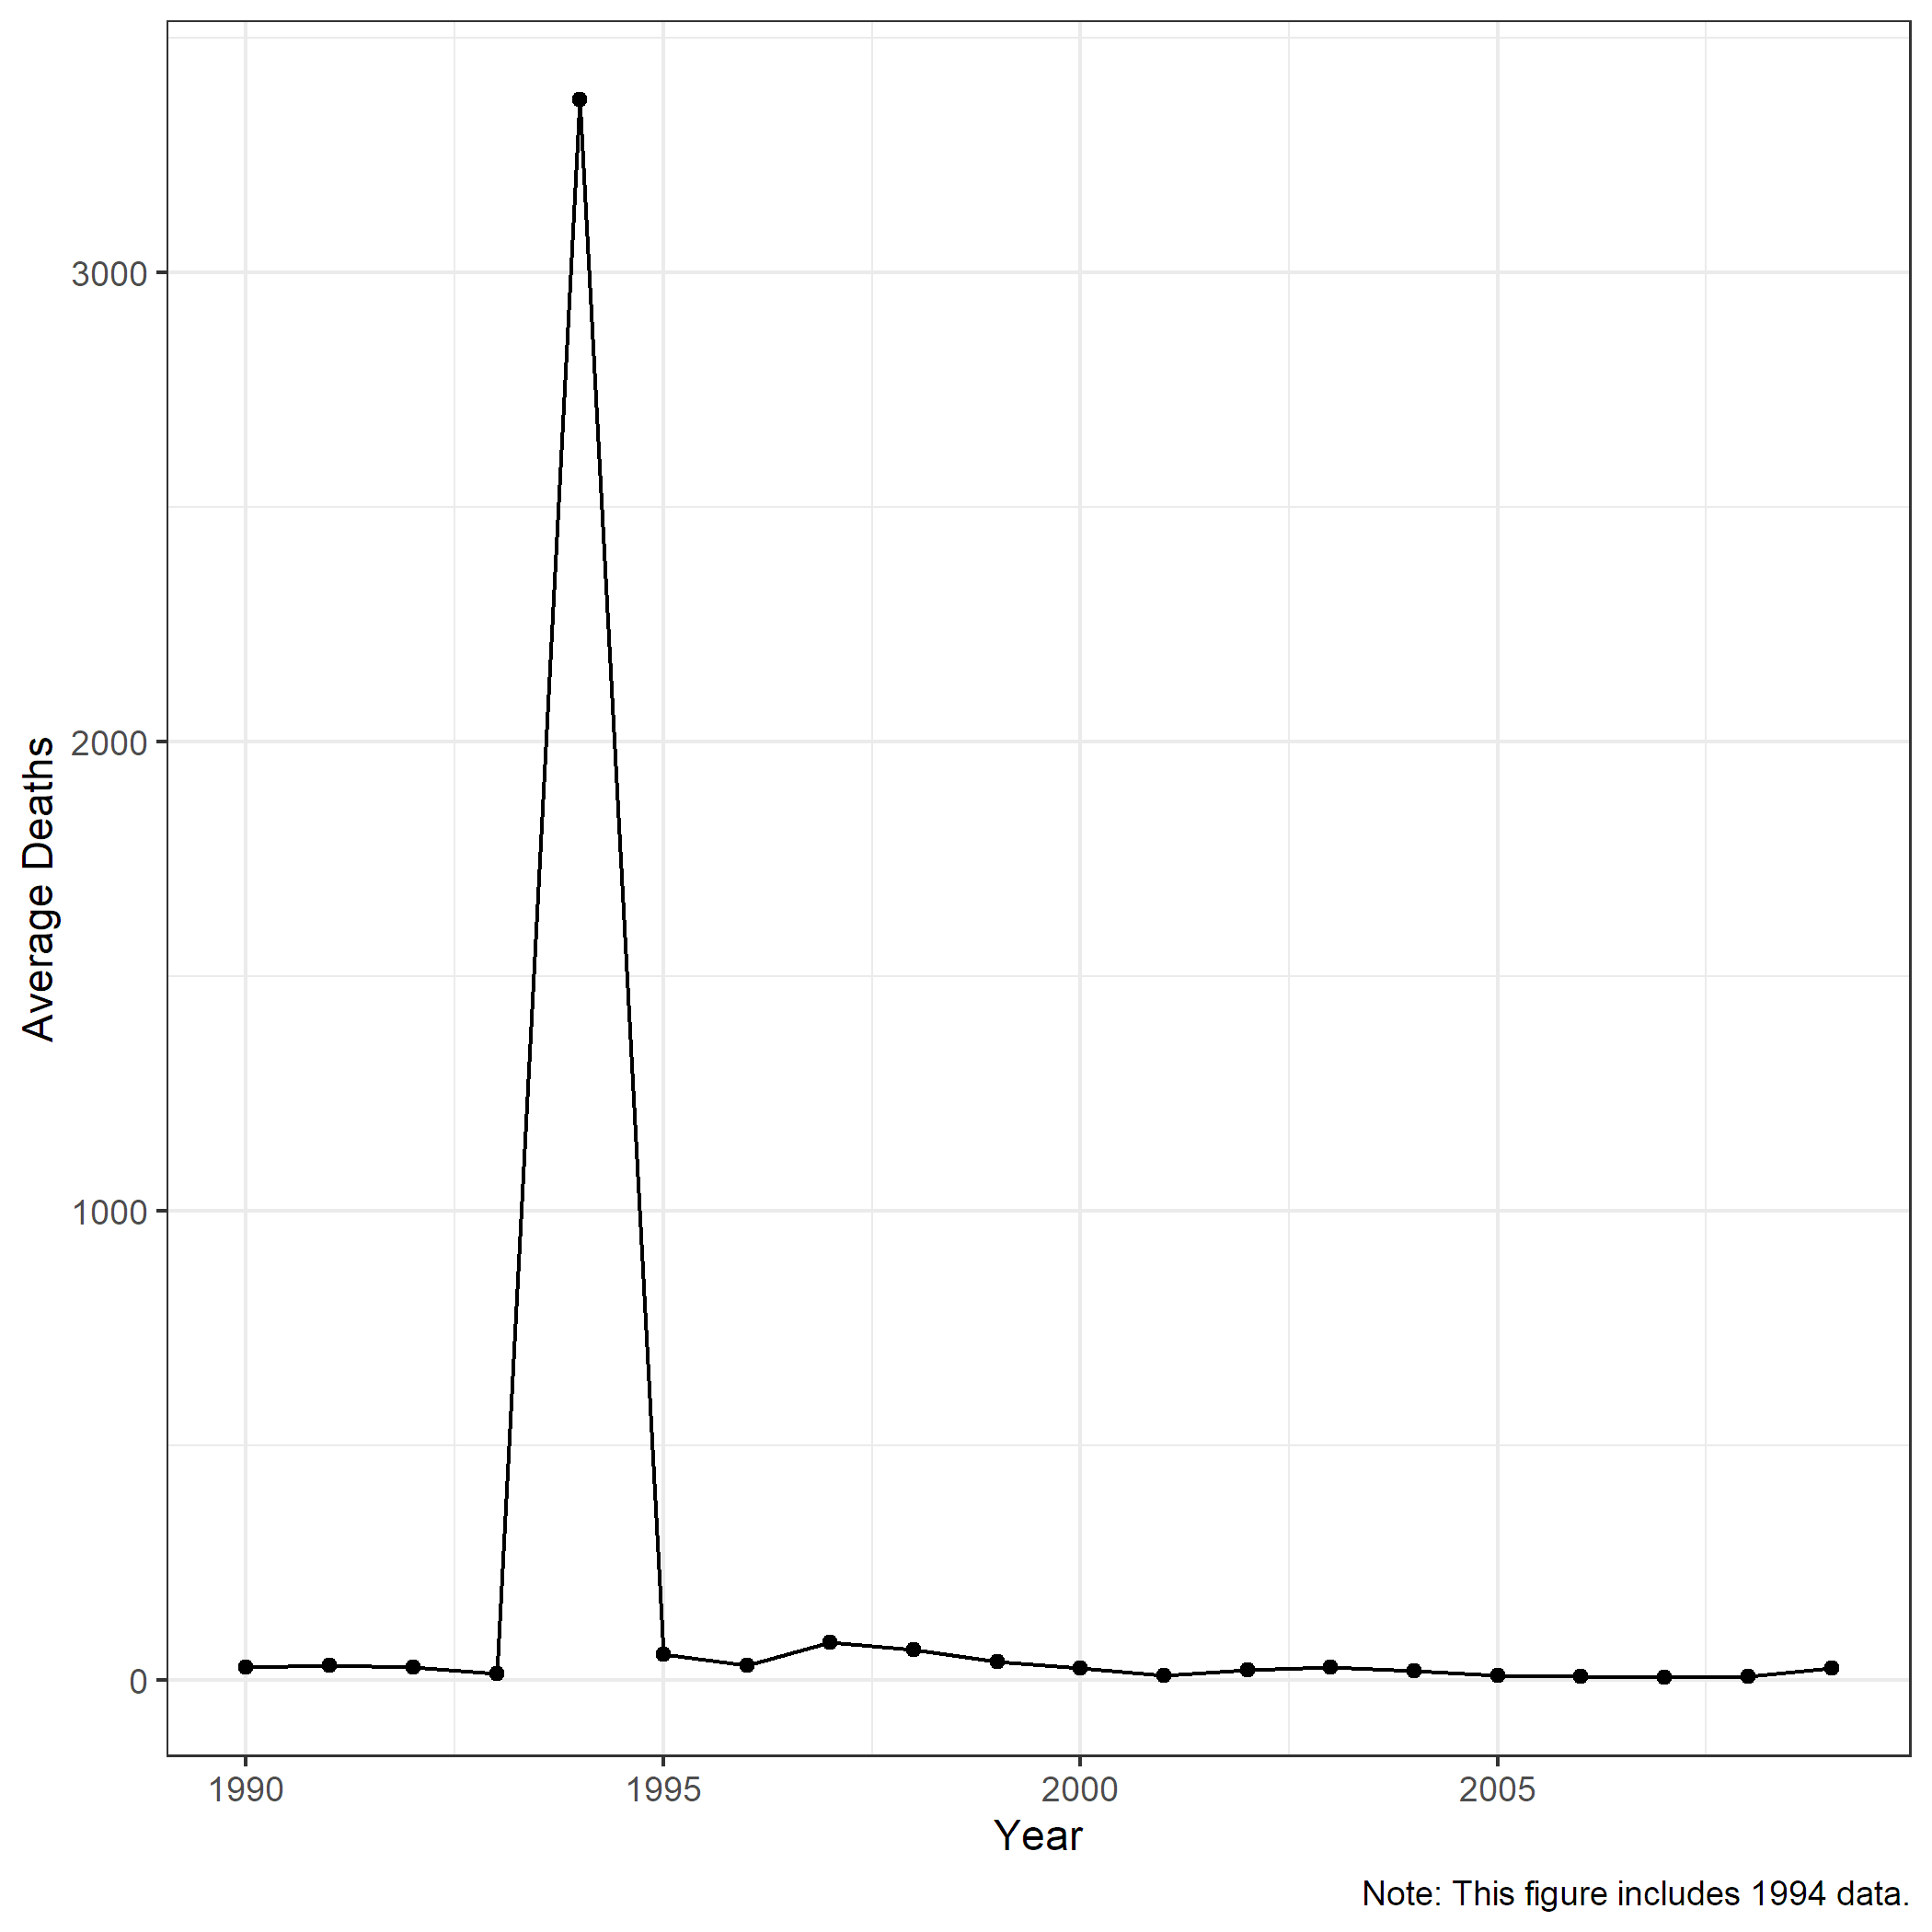
\includegraphics[scale=.8]{appfig4_1}
	\caption{Average of Civilian Deaths Per Year}
\end{figure} 



\clearpage
\phantomsection

{\def\chapter*#1{} % suppress bibliograph header.
\begin{singlespace}
\addcontentsline{toc}{chapter}{REFERENCES}
\begin{center}
{REFERENCES}
\vspace{17pt}
\end{center}


\bibliographystyle{chicago}
\bibliography{MAbib2}

\end{singlespace}




 %updated this

\end{document}
